%\documentclass[12pt,t]{beamer}
\documentclass[xcolor=svgnames]{beamer}

\useoutertheme{infolines}
\usetheme{Boadilla}
%\usetheme[heigth=7mm]{Rochester}
%\usetheme{Rochester}
%\usetheme{Warsaw}
\usecolortheme{whale}


\setbeamertemplate{blocks}[rounded][shadow=true]
\setbeamertemplate{navigation symbols}{}
\usepackage[brazil]{babel}
\usepackage[utf8]{inputenc}
\usepackage{graphicx}
\usepackage{subfigure} 					% uso de várias figuras numa só
\usepackage{algorithm}
\usepackage{algorithmic}
\usepackage{float}

\usepackage{color, colortbl}
%\usepackage[usenames,dvipsnames,svgnames,table]{xcolor}
\usepackage{xcolor}
\usepackage{booktabs}
\usepackage{comment}


%\floatname{algorithm}{Procedure}
\renewcommand{\algorithmicrequire}{\textbf{ \colorbox{yellow}{Input:} }}
\renewcommand{\algorithmicensure}{\textbf{  \colorbox{yellow}{Output:} } }
 \definecolor{keywordColor}{RGB}{165, 42, 42}
 \definecolor{componentColor}{RGB}{0, 0, 205}

\renewcommand{\algorithmicfor}{\textcolor[RGB]{165, 42, 42}{\textbf{For}}}
\renewcommand{\algorithmicendfor}{\textcolor[RGB]{165, 42, 42}{\textbf{End}}}
\renewcommand{\algorithmicdo}{\textcolor[RGB]{165, 42, 42}{\textbf{Do}}}
\renewcommand{\algorithmicreturn}{\textcolor[RGB]{165, 42, 42}{\textbf{Return}}}

\newcommand {\otoprule}{\midrule [\heavyrulewidth]}  % This is for getting a bold horizontal line in the



\bibliographystyle{apalike}
% ------numbering frames-----------------------------------------%
%\newcommand*\oldmacro{}%
%\let\oldmacro\insertshorttitle%
%\renewcommand*\insertshorttitle{%
%	  \oldmacro\hfill%
%	  \insertframenumber\,/\,\inserttotalframenumber
%}
% ---------------------------------------------------------------%

% ------ References ---------------------------------------------%
\usepackage[absolute,overlay]{textpos}
\newenvironment{reference}[2]{%
  \begin{textblock*}{\textwidth}(#1,#2)
      \footnotesize\it\bgroup\color{red!50!black}}{\egroup\end{textblock*}}
% ---------------------------------------------------------------%

\renewcommand{\figurename}{Figura}
\renewcommand{\tablename}{Tabela}

% -------------------------------------------------------------- %
% Pacote necessário para subfiguras
\usepackage{multimedia, multirow}
\graphicspath{{./figures/}}
% -------------------------------------------------------------- %


\title[Defesa de Mestrado]
	%{Monitoramento de coreografias de serviços Web baseado em restrições probabilísticas de QoS  usando SLA}
    {Detecção de Violações de SLA em Coreografias de Serviços Web}
\author[V. A. Phocco-Diaz]
	{
		{\bf Candidato} \\
		Victoriano Alfonso Phocco Diaz \\%\footnote{O aluno recebeu apoio financeiro do CNPq, processo 133147/2009-6} \\ [1ex]
		{\bf Orientador} \\  Daniel Macêdo Batista 	\\
		%%{\bf Co-orientador} \\  Marco Dimas Gubitoso 	
	}
\institute[IME-USP]
	{Instituto de Matemática e Estatística \\
	 Departamento de Ciência da Computação \\	
	 Universidade de São Paulo  \\  [1ex]
	 %\texttt{alfonso7@ime.usp.br}
	}
\date[Março 2013]{Março de 2013}
%\date[]{}



%%% Slides ---------------------------------
\begin{document}
%\pgfdeclareimage[width=180pt,height=20pt]{test}{images/header.jpg}
%\logo{\pgfuseimage{test}}

% --- the titlepage frame ------------------------------------------%
\begin{frame}[plain]
\titlepage
\end{frame}

\section*{Roteiro}
    \begin{frame}{Roteiro}
        \tableofcontents[subsectionstyle=hide]
    \end{frame}

% ------------------------------------------------------------------%
\AtBeginSection[]
{
	\begin{frame}<beamer>
		\frametitle{}
		\tableofcontents[currentsection,%, currentsubsection
		  sectionstyle=show/shaded,
		  %hideothersubsections
		  %subsectionstyle=hide, 
		  %hideallsubsections
		  %subsectionstyle=show/shaded, 
		]
	\end{frame}
}

\AtBeginSubsection[]{
  \frame{
  \tableofcontents[currentsection,currentsubsection,hideothersubsections,subsectionstyle=show/shaded ]
  }
}
% ------------------------------------------------------------------%
% ------------------------------------------------------------------%
% ---------------------- Problema    -------------------------------%
\section{Conceitos Básicos}

% -----  Serviços Web ----------%
    \begin{frame}{Serviço Web}
    	Definição pela W3C [W3C,2004]: %\cite{W3C2004}:
    	\begin{block}{Serviço Web}\vspace{-.3\baselineskip}
        	 \begin{quote}
                 A Web service is a software system designed to support interoperable machine-to-machine interaction over a network. It has an
 interface described in a machine-processable format (specifically WSDL). Other systems interact with the Web service in a manner
prescribed by its description using SOAP messages, typically conveyed using HTTP with an XML serialization in conjunction with other Web-related standards.
        	 \end{quote}
    	\end{block}
	%%Tecnologias
     \tiny{
        %\begin{thebibliography}{1}
        %  \beamertemplatearticlebibitems
          %\bibitem[W3C,2004]{W3C2004}
           % Web Services Architecture Working Group {\em Web Service Architecture}.
            %W3C Working Group Note 11. 2004. \url{http://www.w3.org/TR/ws-arch/}. Último acesso em 07-09-2011.
            %\newblock {\em Bootstrapping Performance and Dependability Attributes of Web Services}.
            %\newblock IEEE International Conference on Web Services (ICWS'06). 2006:205-212.
       %\end{thebibliography}
      }
    \end{frame}

% -----  SOA ----------%
    \begin{frame}{SOA (1/2)}
            \begin{block}{SOA (Arquitetura Orientada a Serviços)}\vspace{-.3\baselineskip}
            É um estilo de arquitetura de software cujo princípio fundamental prega que as funcionalidades implementadas pelas
	    aplicações devem ser disponibilizadas na forma de serviços [SOA, 2006]. %\cite{SOA2006}.
            \end{block}

            \tiny{
                %\begin{thebibliography}{0}
                 %         \beamertemplatearticlebibitems
                 % \bibitem[SOA,2006]{SOA2006}
                  %  SOA Working Group of The Open Group. {\em Definition of SOA}.
                  %  2006. \url{http://www.opengroup.org/projects/soa/}.Último acesso em 01-10-2011.
                    %\newblock {\em Bootstrapping Performance and Dependability Attributes of Web Services}.
                    %\newblock IEEE International Conference on Web Services (ICWS'06). 2006:205-212.
               %\end{thebibliography}
            }
    \end{frame}

    \begin{frame}{SOA (2/2)}
         \only<1>{	
              \begin{figure}[!h]
                  \centering
                  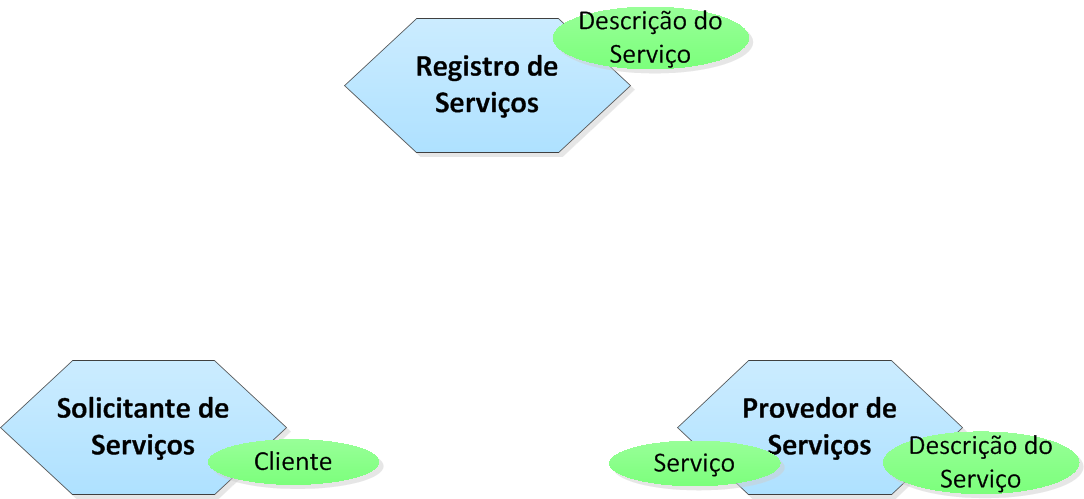
\includegraphics[width=0.9\textwidth]{SOA-Triangle_1.png}
                  \caption{Triângulo da SOA (baseado em [W3C, 2002])}
              \end{figure}	
          }
          \only<2>{	
              \begin{figure}[!h]
                  \centering
                  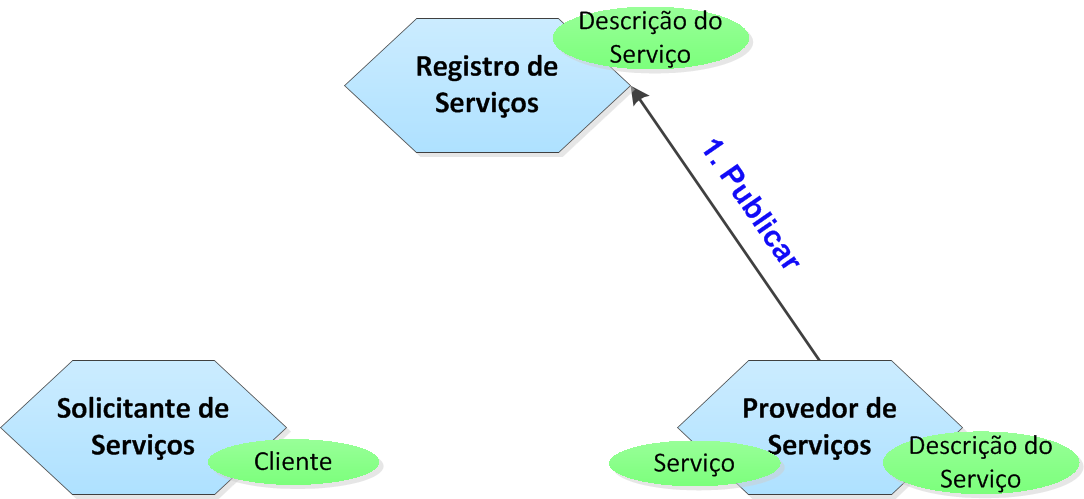
\includegraphics[width=0.9\textwidth]{SOA-Triangle_2.png}
                  \caption{Triângulo da SOA (baseado em [W3C, 2002])}
              \end{figure}	
          }
          \only<3>{	
              \begin{figure}[!h]
                  \centering
                  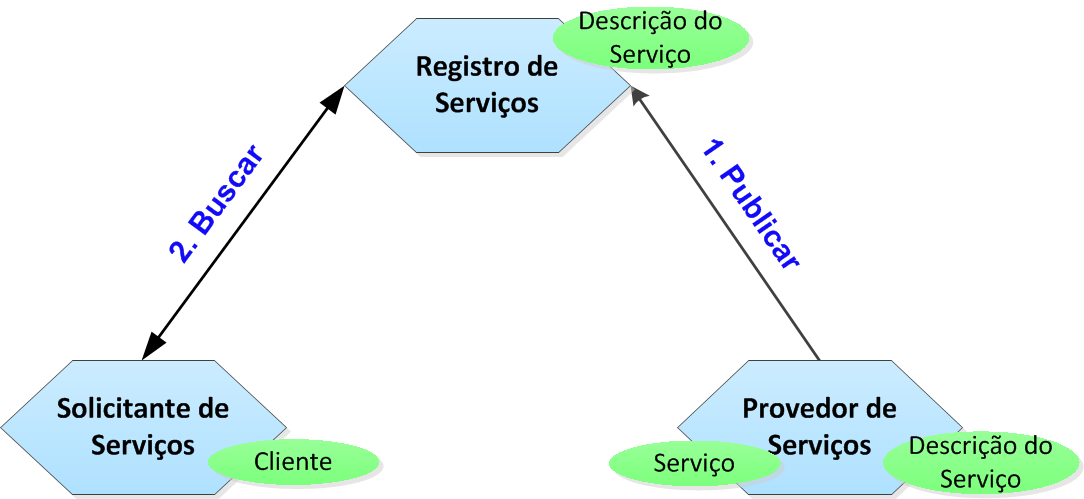
\includegraphics[width=0.9\textwidth]{SOA-Triangle_3.png}
                  \caption{Triângulo da SOA (baseado em [W3C, 2002])}
              \end{figure}	
          }

          \only<4>{	
              \begin{figure}[!h]
                  \centering
                  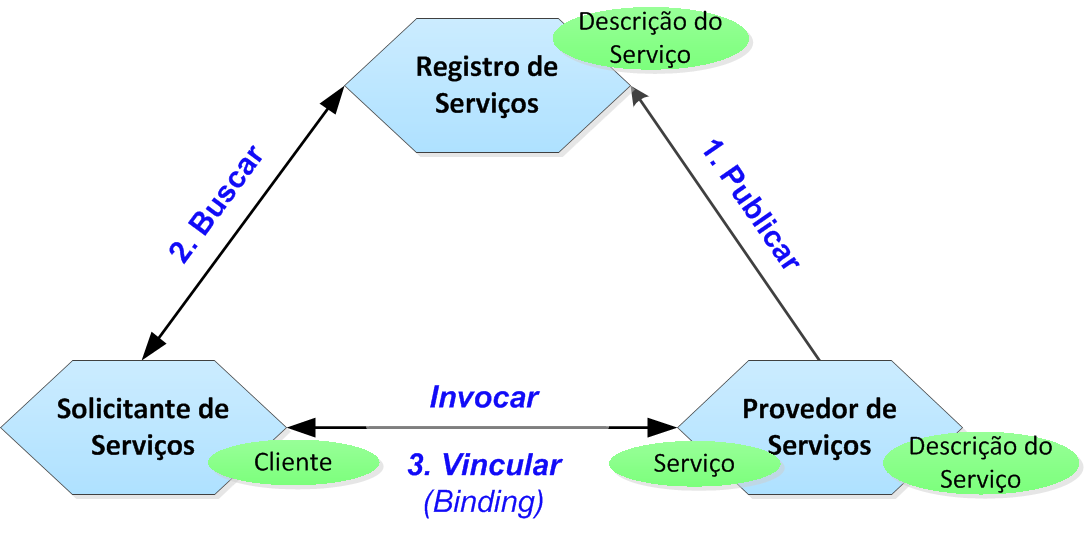
\includegraphics[width=0.9\textwidth]{SOA-Triangle_4.png}
                  \caption{Triângulo da SOA (baseado em [W3C, 2002])}
              \end{figure}	
          }
          \only<5>{	
              \begin{figure}[!h]
                  \centering
                  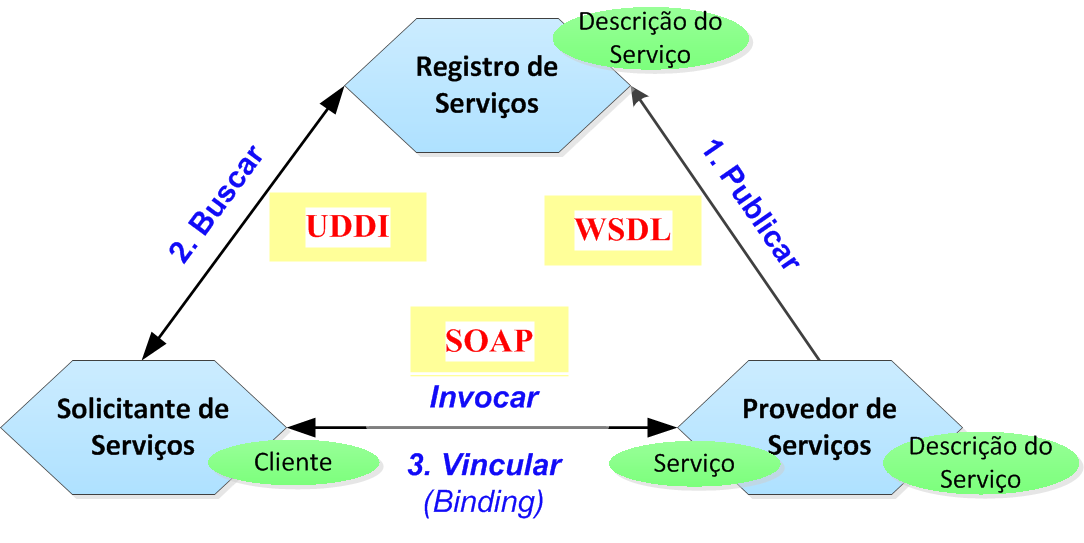
\includegraphics[width=0.9\textwidth]{SOA-Triangle_5.png}
                  \caption{Triângulo da SOA (baseado em [W3C, 2002])}
              \end{figure}	
          }

    \end{frame}

% -----  SOC ----------%
    \begin{frame}{SOC}
       	\begin{block}{SOC (Computação Orientada a Serviços)}\vspace{-.3\baselineskip}
           É um novo paradigma de computação que utiliza serviços como blocos básicos de construção
           para suportar o desenvolvimento rápido, de baixo custo e de fácil composição de aplicações
           distribuídas heterogêneas [Papazoglou et al., 2006]. %\cite{Papazoglou2007}.
        \end{block}
        Elementos Chave:

        \begin{itemize}
           \item Serviços.
           \item SOA.
           \item Composição de Serviços.
           \item QoS.
        \end{itemize}


        \tiny{
            %\begin{thebibliography}{3}
             %         \beamertemplatearticlebibitems
             % \bibitem[Papazoglou et al., 2006]{Papazoglou2007}
             %   Papazoglou MP, Traverso P, Dustdar S, Leymann F. {\em Service-Oriented Computing: a Research Roadmap}.
             %   International Journal of Cooperative Information Systems. 2008;17(02):223.
                %\newblock {\em Bootstrapping Performance and Dependability Attributes of Web Services}.
                %\newblock IEEE International Conference on Web Services (ICWS'06). 2006:205-212.
           %\end{thebibliography}
        }
        	
      %Adicionar padrões
    \end{frame}


% -----  Composição de Serviços ----------%
    \begin{frame}{Composição de Serviços}
        \begin{itemize}
          \item \textbf{Serviço Composto}: Um serviço construído a partir de outros serviços. O serviço composto também é um serviço.
          \item \textbf{Composição de Serviços}: Processo de  obter serviços compostos combinando e vinculando outros serviços.
          \item <1->Abordagens:
                \begin{itemize}
                  \item <2->\colorbox{yellow}{\textbf{Orquestração de Serviços}}.
                  \item <3->\colorbox{yellow}{\textbf{Coreografia de Serviços}}.
                \end{itemize}
        \end{itemize}
    \end{frame}

    %----- Orquestração de Serviços -----%
    \begin{frame}{Orquestração de Serviços}
          \only<1>{	
              \begin{figure}[!h]
                  \centering
                  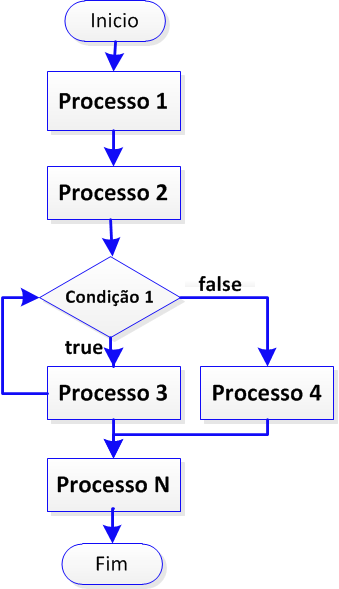
\includegraphics[width=0.25\textwidth]{Orchestration_1.png}
                  \caption{Orquestração de serviços}
              \end{figure}	
          }
          \only<2>{	
              \begin{figure}[!h]
                  \centering
                  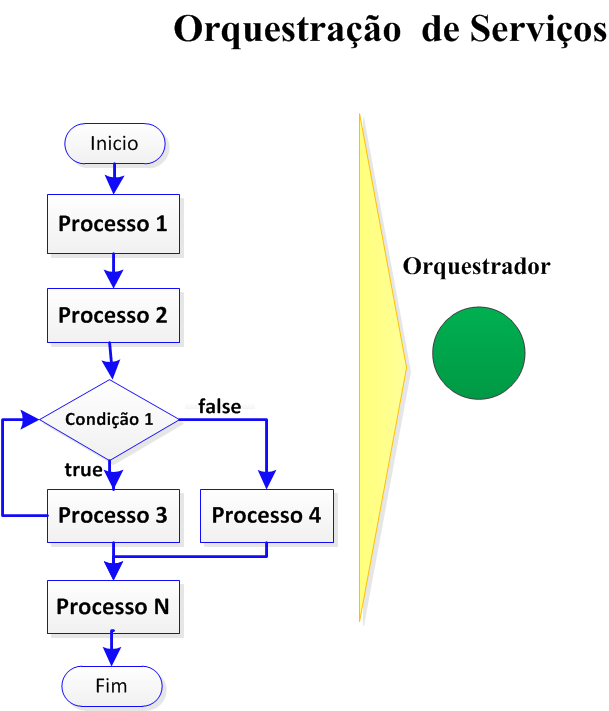
\includegraphics[width=0.45\textwidth]{Orchestration_2.png}
                  \caption{Orquestração de serviços}
              \end{figure}	
          }
          \only<3>{	
              \begin{figure}[!h]
                  \centering
                  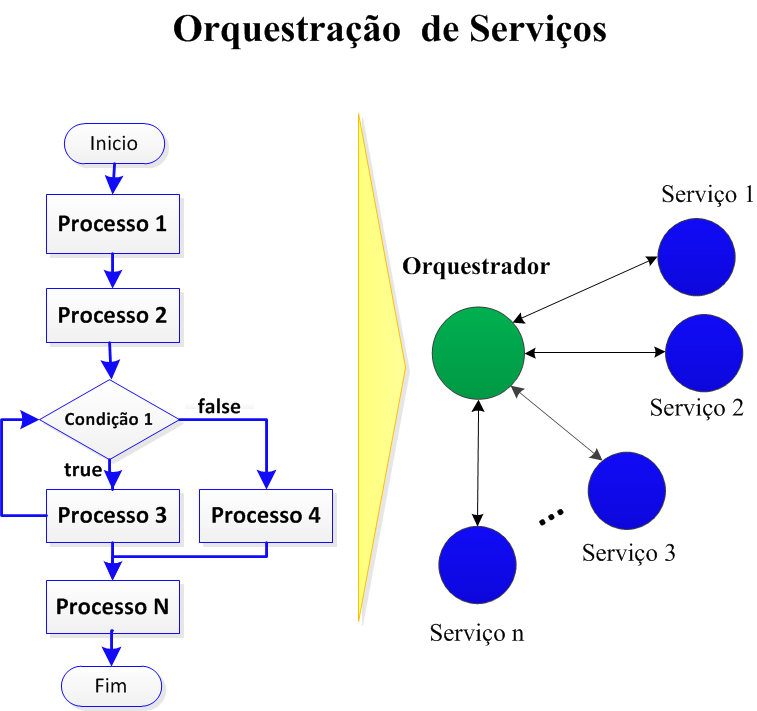
\includegraphics[width=0.5\textwidth]{Orchestration_3.png}
                  \caption{Orquestração de serviços}
              \end{figure}	
          }
         % \only<4>{	
         %     \begin{figure}[!h]
         %         \centering
         %         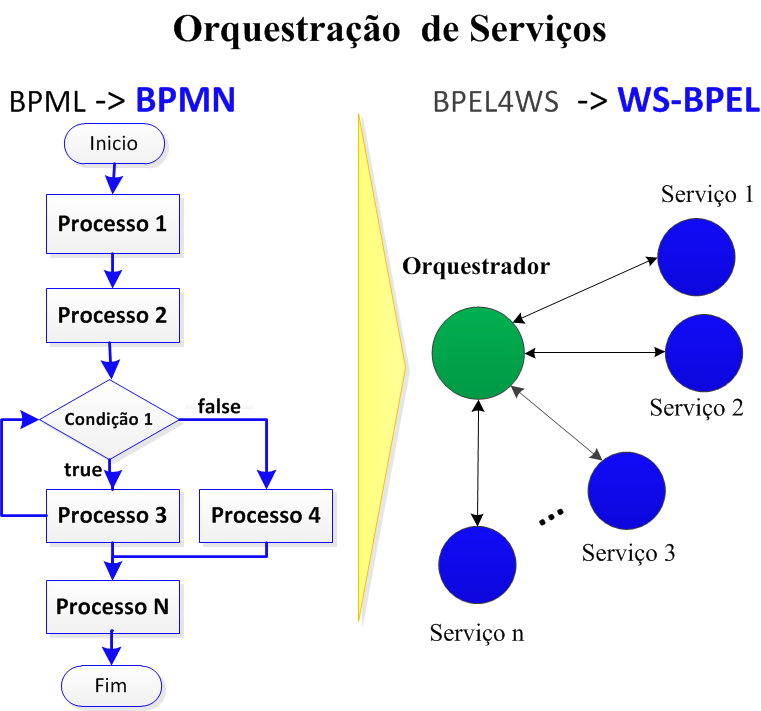
\includegraphics[width=0.5\textwidth]{Orchestration_4.png}
         %         \caption{Orquestração de serviços}
         %     \end{figure}	
         % }


    \end{frame}


    %----- Coreografia de Serviços -----%
    \begin{frame}{Coreografia de Serviços}
          \only<1>{	
              \begin{figure}[!h]
                  \centering
                  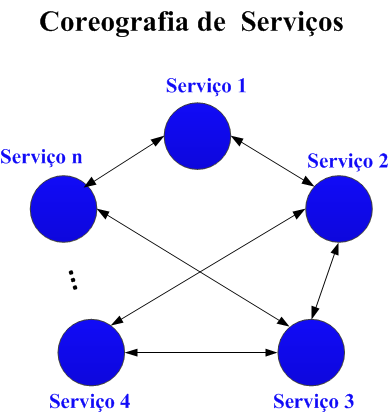
\includegraphics[width=0.5\textwidth]{ChoreographyA.png}
                  \caption{Coreografia de serviços}
              \end{figure}	
          }
          %\only<2>{	
           %   \begin{figure}[!h]
            %      \centering
            %      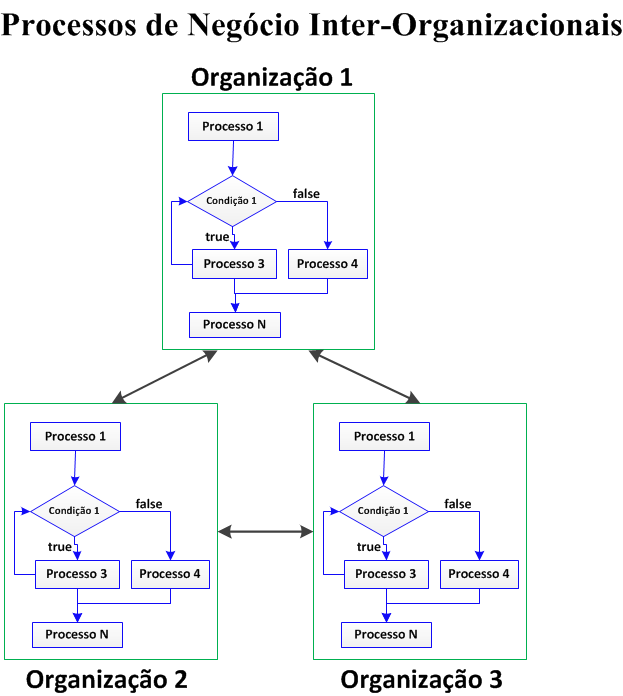
\includegraphics[width=0.6\textwidth]{ChoreographyB_1.png}
            %      \caption{Coreografia de serviços}
            %  \end{figure}	
          %}
          \only<2>{	
              \begin{figure}[!h]
                  \centering
                  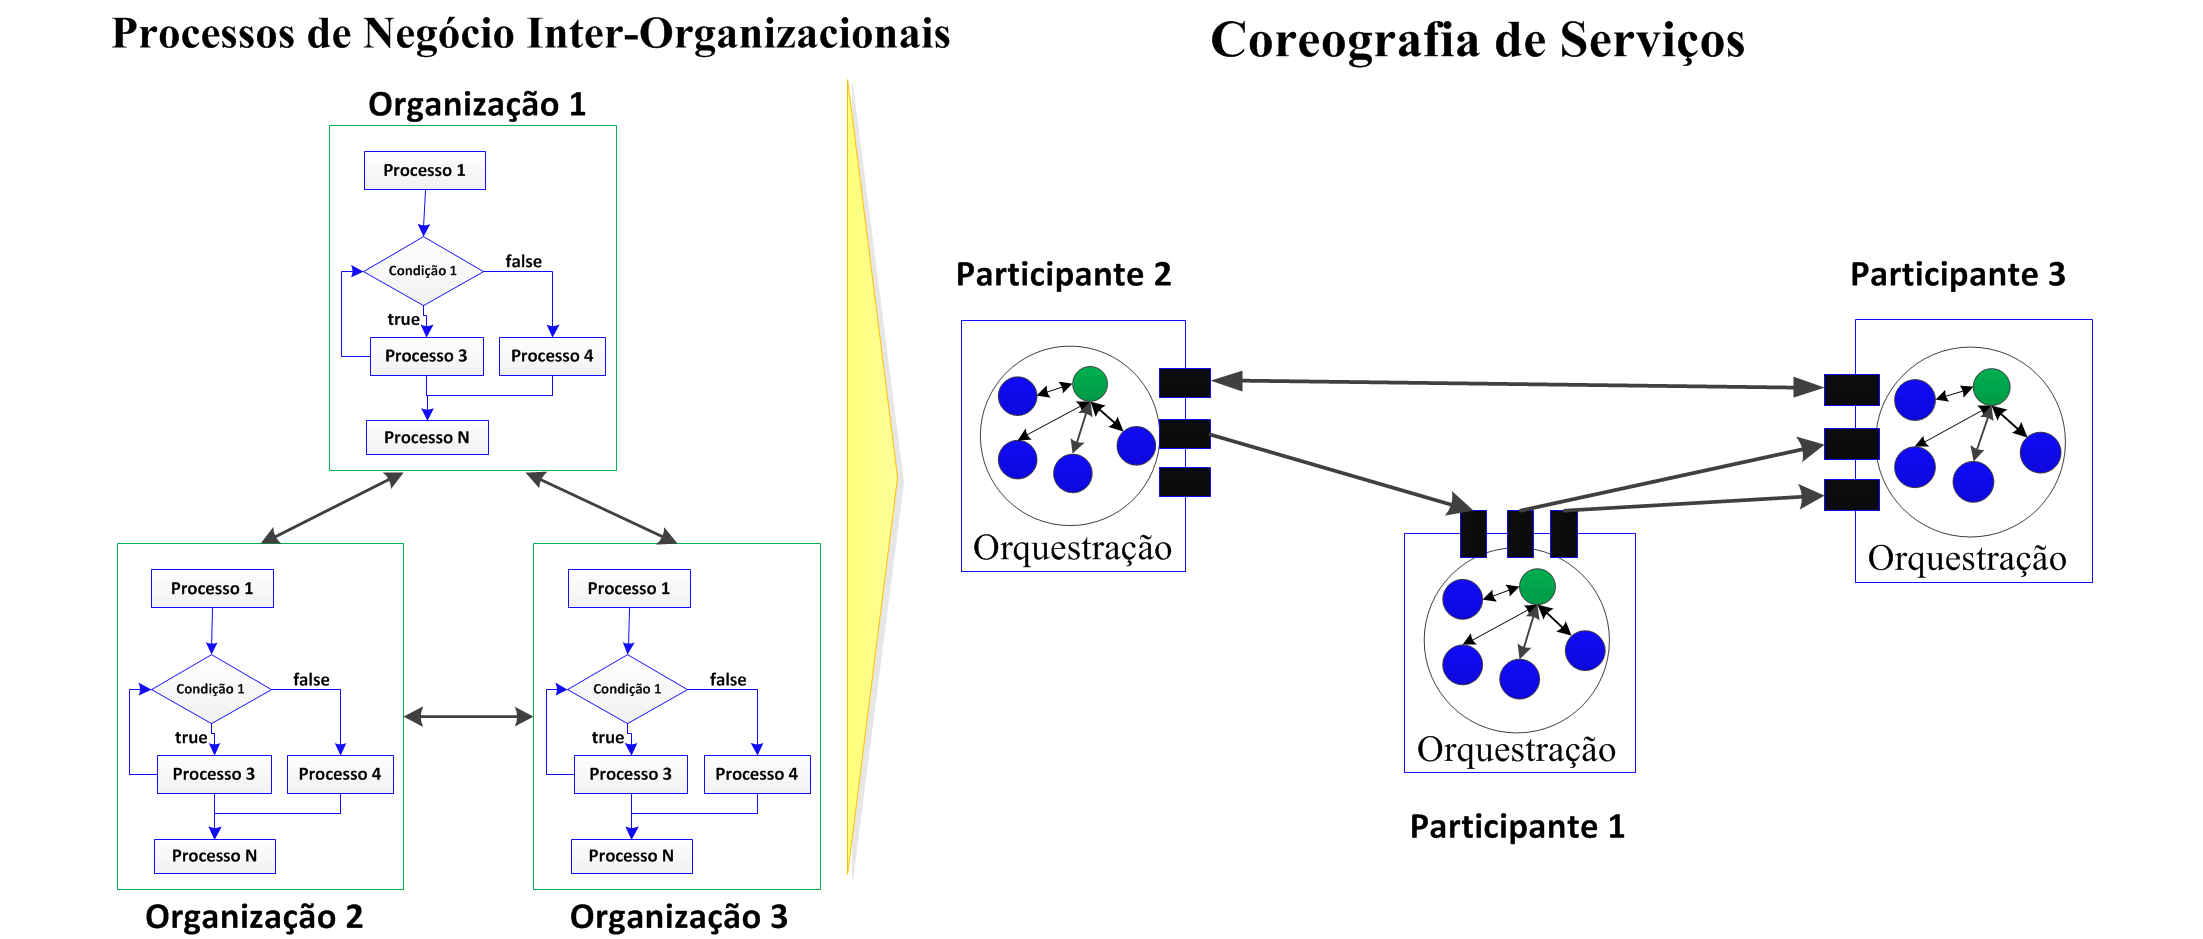
\includegraphics[width=1.0\textwidth]{ChoreographyB_2.png}
                  \caption{Coreografia de serviços}
              \end{figure}	
          }
          \only<3>{	
              \begin{figure}[!h]
                  \centering
                  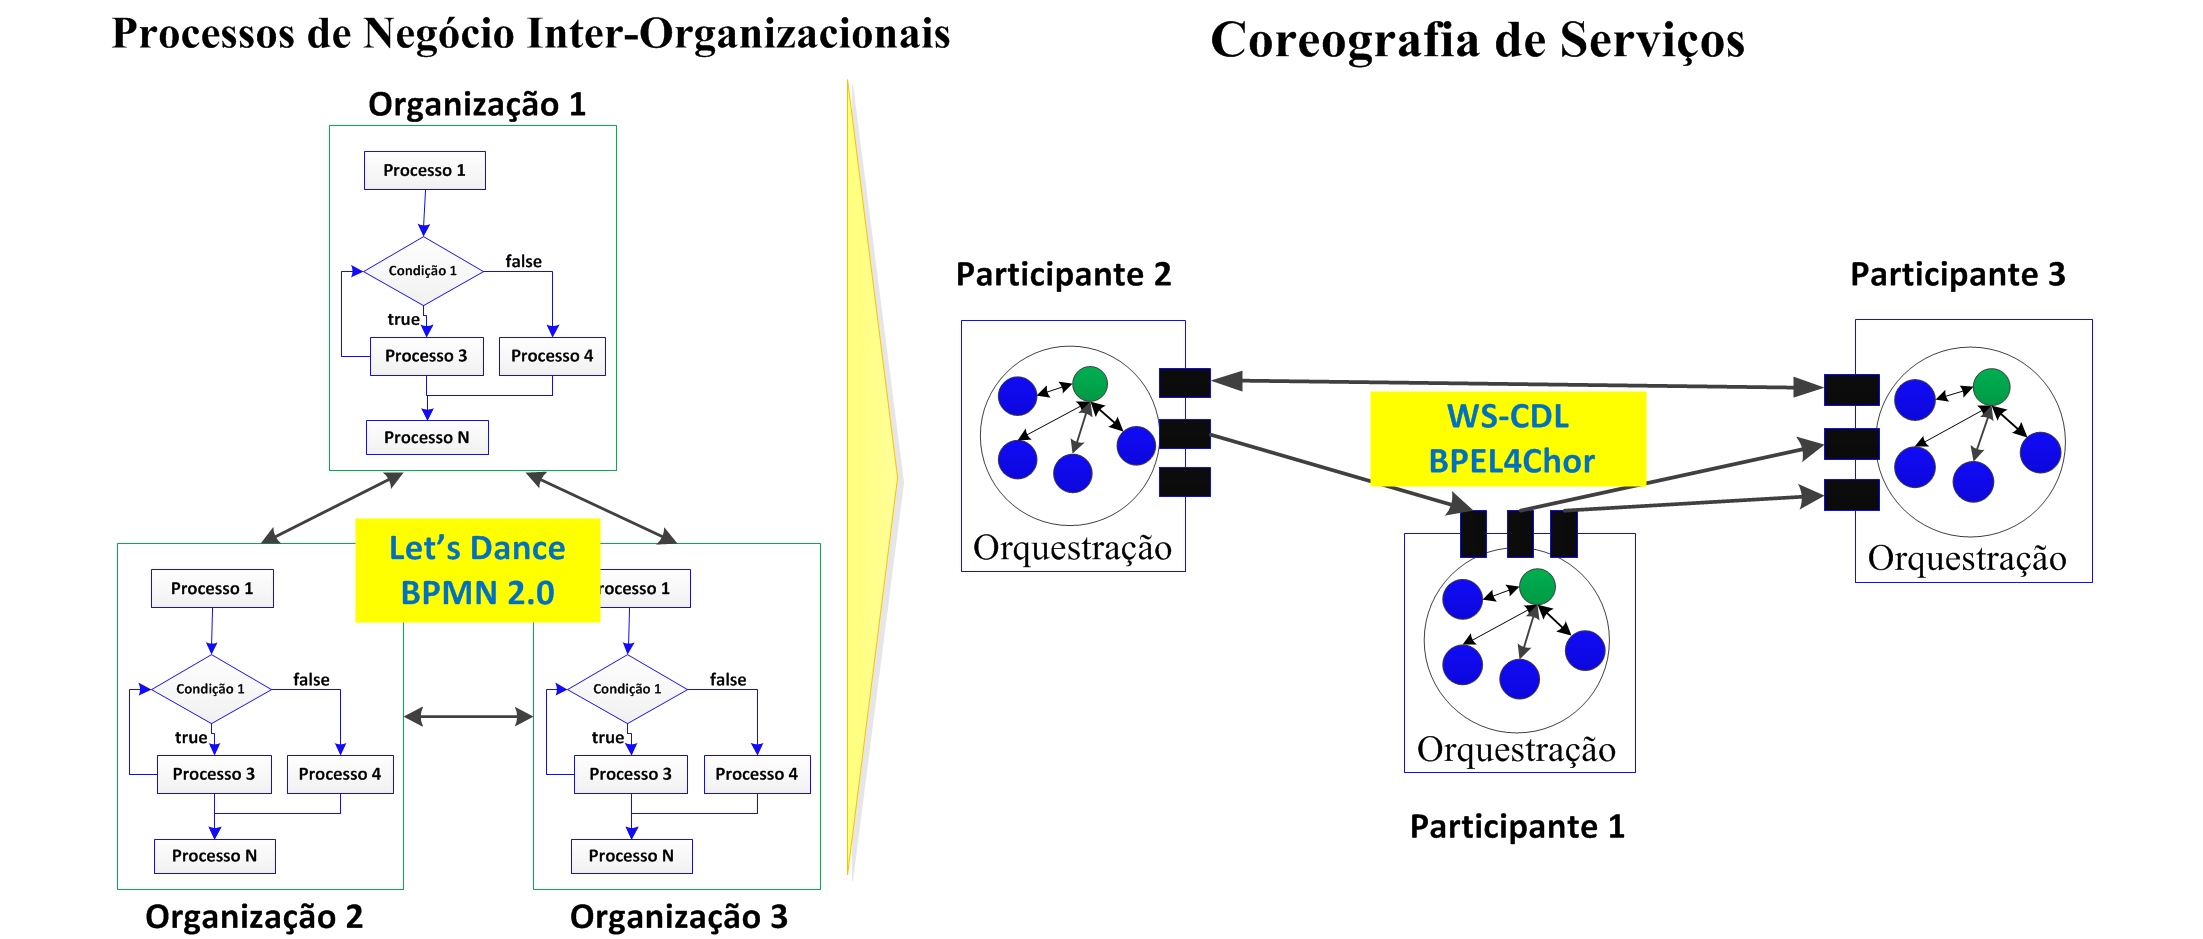
\includegraphics[width=1.0\textwidth]{ChoreographyB_3.png}
                  \caption{Coreografia de serviços}
              \end{figure}	
          }
    \end{frame}

    \begin{frame}{Coreografia de Processos}
      \begin{itemize}
	%\item <1-> A Choreography is specified in BPMN 2.0 (Process Choreography).
	  %\begin{itemize}
	  %  \item Differs in purpose and behavior from a standard BPMN Process (Process Orchestration).
	    %\item Formalizes the way business \colorbox{yellow}{Participants} \textbf{coordinate} their \colorbox{yellow}{interactions}.
	  % \item Formalizes the way business \textcolor{blue}{\textbf{Participants}} \textbf{coordinate} their \textcolor{blue}{\textbf{interactions}}.
	  %\end{itemize}
	%\item <2-> Focus on the exchange of information (\colorbox{yellow}{Messages}) between these Participants.
	%\item <1-> Focus on interactions through \textcolor{blue}{\textbf{messages exchanges}}.
	\item <1-> Uma Coreografia também é um processo.
	\item <2-> \textbf{BPMN} (Bussiness Process Model and Notation) é um padrão para modelagem de processo de negócios.
	\item <2-> \textbf{BPMN} suporta modelagem de coreografias.
	\item <3-> Duas abordagens de modelagem:
	  \begin{itemize}
	    \item <3-> \colorbox{yellow}{Modelo de Interconexão}%: With collaborations diagrams.
	    \item <4-> \colorbox{yellow}{Modelo de Interação}%:  BPMN Choreographies. using special activities (\textit{Choreography Activity}).
	  \end{itemize}
      \end{itemize}

    \end{frame}


  \begin{frame}{Modelo de Interconexão }
      \begin{itemize}
	\item Vistas públicas interconectadas.	
	\item Uso de atividades de processos comuns.
 	\item Colaborações em BPMN 2.
      \end{itemize}
   \begin{figure}[!h]
	    \centering
	    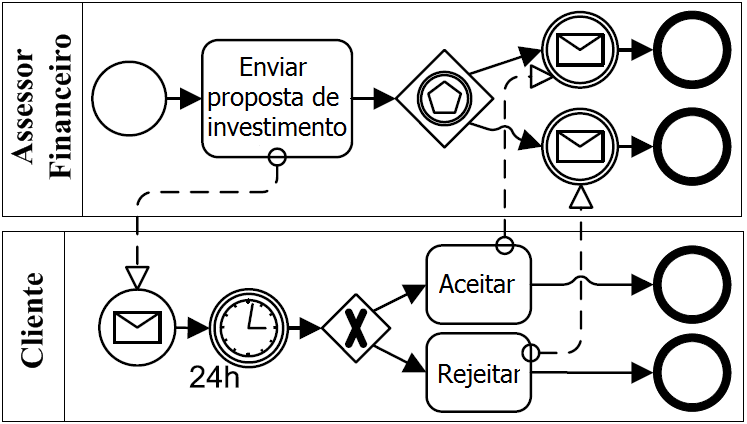
\includegraphics[width=0.6\textwidth]{figures/interconnection_choreography-pt.png}
	    %\caption{BPMN elements for modeling choreographies.}
    \end{figure}	
  \end{frame}

  \begin{frame}{ Modelo de Interação}
    \begin{itemize}
	  \item Interações \textbf{capturadas globalmente}.	
	  \item Blocos básicos de construção: \textbf{interações atômicas} entre participantes.
	  \item Suportado a partir do BPMN 2.
	\end{itemize}
    \begin{figure}[!h]
	      \centering
	      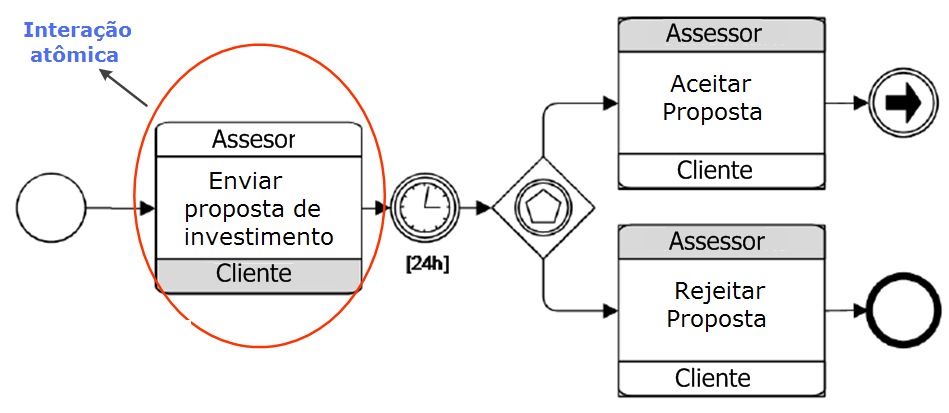
\includegraphics[width=0.7\textwidth]{figures/interaction_choreography2-br.png}
	      %\caption{BPMN elements for modeling choreographies.}
      \end{figure}	
  \end{frame}


    %----- Categorização de Coreografias -----%
    %\begin{frame}{Classificação das Linguagens de Coreografias}
    %  \begin{figure}[!h]
    %      \centering
    %      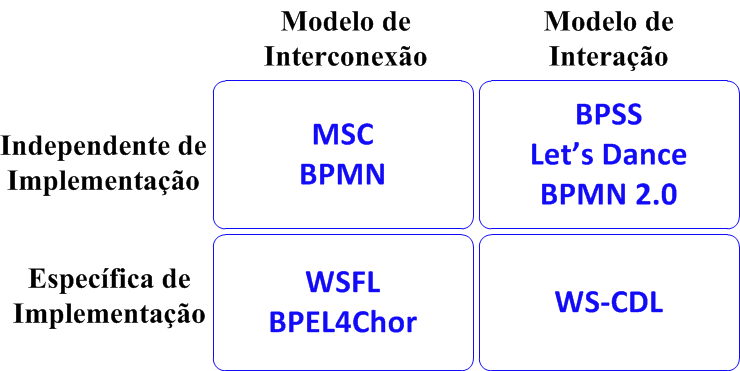
\includegraphics[width=0.7\textwidth]{ChoreographyCategorization.png}
    %      \caption{Classificação das linguagens de coreografias }
    %  \end{figure}	
    %\end{frame}




% ------------------------------------------------------------------%
% ------------------------------------------------------------------%
% -------------------- Objetivos------------------------------------%
\section{Problema}

    \begin{frame}{Objetivos}
        \begin{block}{Objetivo principal}\vspace{-.3\baselineskip}
        	\begin{itemize}
                  %\item Propor uma técnica de monitoramento ``não intrusivo'' de coreografias de serviços Web usando SLAs.
        		  %\item Propor uma técnica para definir SLAs baseado em restrições probabilísticas de QoS.
                  \item Detectar violações de SLAs em coreografias de serviços web.
            \end{itemize}
        \end{block}
        \begin{block}{Objetivos secundários}\vspace{-.3\baselineskip}
        	\begin{itemize}
        	      %\item Realizar a implementação do monitoramento ``não intrusivo''.
		  \item	Propor uma técnica para definir SLAs baseada em restrições probabilísticas de QoS.
                  \item Propor e implementar uma técnica de monitoramento ``não intrusivo'' de coreografias
                    de serviços Web usando SLAs.
                  %\item Realizar avaliações da técnica de monitoramento.
                  \item Avaliar o desempenho das propostas. %técnica de monitoramento.
        	\end{itemize}
        \end{block}
    \end{frame}

    \begin{frame}{Justificativa}
    	\begin{itemize}
          \item <1->Importância da \textbf{coreografia} de serviços Web.
          \item <2->\textbf{QoS} é um fator importante na adaptação, seleção, otimização, composição na SOC. %\footnote{SOC: Computação Orientada a Serviços}.
          \item <3->\textbf{Monitoramento} é uma base para a reação (adaptação, reconfiguração, renegociação, etc).
              	\begin{itemize}
                  \item Detecção de falhas e violações de SLA. %\footnote{SLA: Acordo de Nível de Serviço}.
                \end{itemize}
          %\item <4->Monitoramento em tempo de execução Vs.  verificações e validações estáticas.
          \item <4->\textbf{Contratos probabilísticos} refletem melhor o comportamento dinâmico dos \textbf{atributos de QoS} dos serviços Web.
    	\end{itemize}
    \end{frame}

    %----- Coreografia de Serviços -----%
    \begin{frame}{Problema a ser resolvido}
      \begin{figure}[!h]
	  \centering
	  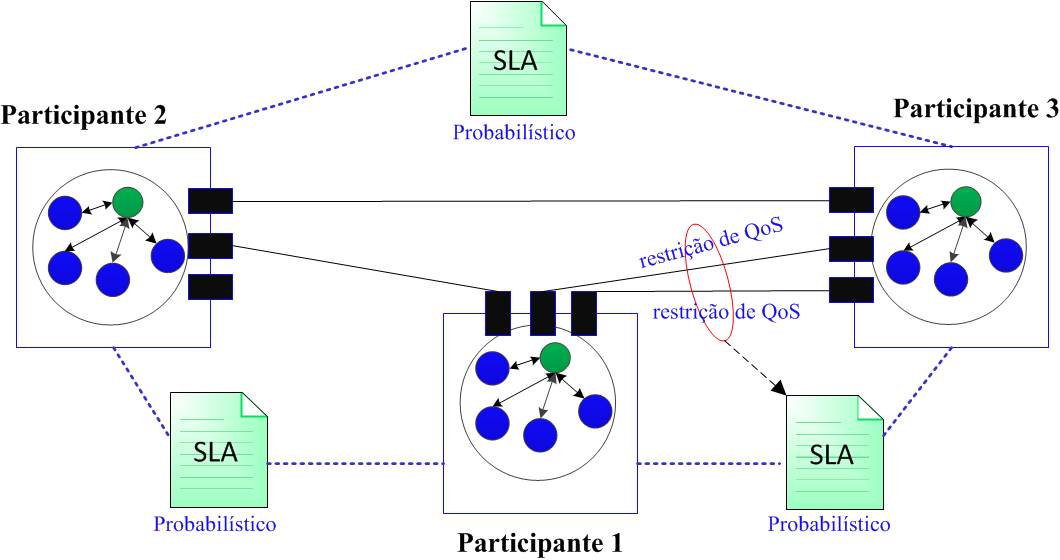
\includegraphics[width=0.8\textwidth]{ChoreographySLAs.png}
	  \caption{Problema a ser resolvido}
      \end{figure}	
    \end{frame}





% ------------------------------------------------------------------%
% ------------- Monitoramento baseado em QoS -----------------------%
% ------------------------------------------------------------------%
\section{QoS e Monitoramento em Coreografias de Serviços Web }

    %----- Coreografia de Serviços -----%
    \begin{frame}{Problema a ser resolvido}
      \begin{figure}[!h]
	  \centering
	  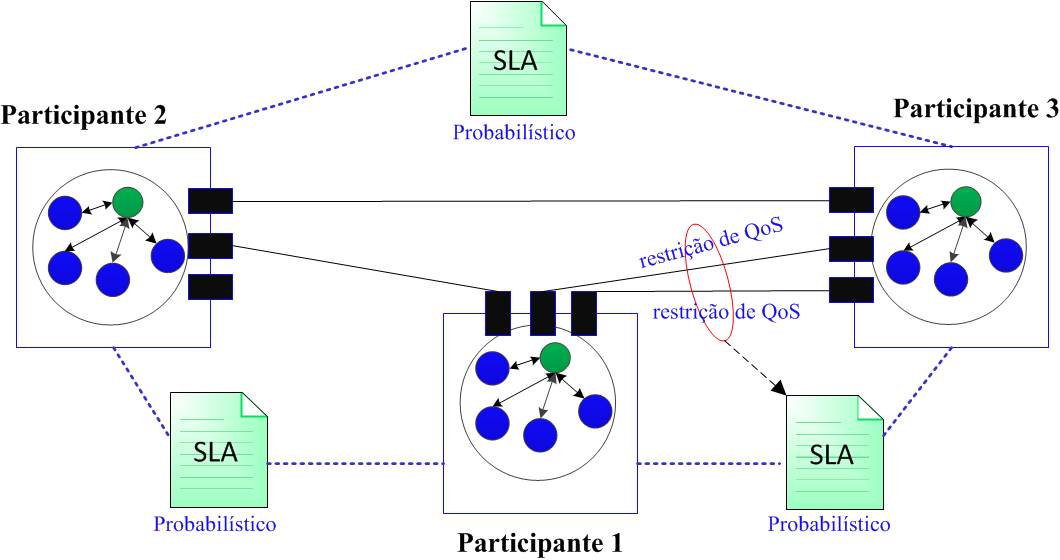
\includegraphics[width=0.8\textwidth]{ChoreographySLAs.png}
	  \caption{Problema a ser resolvido}
      \end{figure}	
    \end{frame}

%\subsection{ QoS e SLA}
%----- Qualidade de Serviços -----
    \begin{frame}{Qualidade de Serviço}
        \begin{itemize}
          \item Qualidade de Serviço : QoS.
          \item \textbf{Funcionalidade/serviço} = Quais operações o sistema executa.
                \begin{itemize}
                    \item Exemplo: compra de passagens de avião.
                \end{itemize}

          \item \textbf{QoS/Característica Não Funcional} = Quão bem o sistema executa os serviços.
                \begin{itemize}
                    \item Exemplo: O tempo médio de resposta é 2 segundos.
                \end{itemize}
          \item Importante em Composição de Serviços : \textbf{\emph{QoS-aware Composition}}.
        \end{itemize}
  \end{frame}

%---------- Qualidade de Serviço ---------
    \begin{frame}{Qualidade de Serviço}
      \begin{figure}[!h]
          \centering
          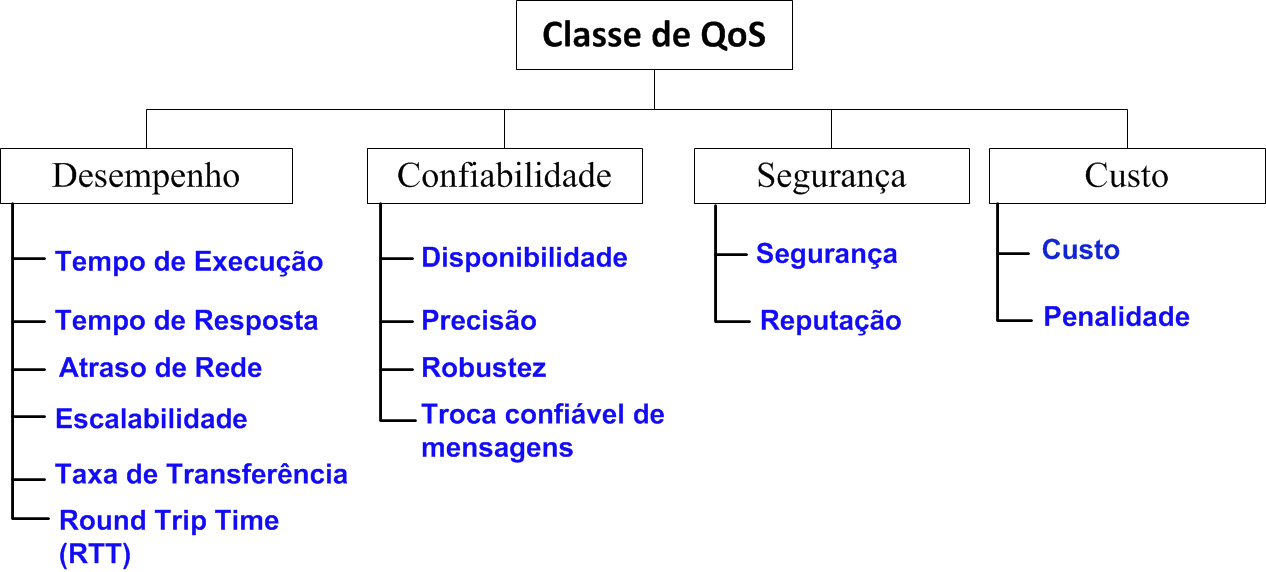
\includegraphics[width=1.0\textwidth]{QoSTaxonomy.png}
          \caption{Taxonomia de atributos de QoS [Rosenberg et al.,2006] } %\cite{Rosenberg2006}}
          %\label{fig:QoST_SLA_Mapping_Transformation}
      \end{figure}	

      \tiny{
        %\begin{thebibliography}{4}
         %         \beamertemplatearticlebibitems
         %  \beamertemplatearticlebibitems
         % \bibitem[Rosenberg et al.,2006]{Rosenberg2006}
          %  Rosenberg F, Platzer C, Dustdar S. {\em Bootstrapping Performance and Dependability Attributes of Web Services}.
          %  IEEE International Conference on Web Services (ICWS’06). 2006:205-212.
            %\newblock {\em Bootstrapping Performance and Dependability Attributes of Web Services}.
            %\newblock IEEE International Conference on Web Services (ICWS’06). 2006:205-212.
       %\end{thebibliography}
      }
    \end{frame}

%---------- Cálculo de Qos ---------
    \begin{frame}{Cálculo de QoS}
      \only<1>{	
          \begin{figure}[!h]
              \centering
              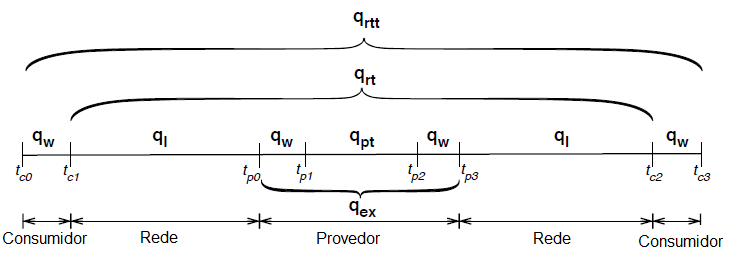
\includegraphics[width=1.0\textwidth]{ServiceInvocationTimes_.png}
              \caption{Instantes de tempo na utilização de um serviço Web [Michlmayr et al.,2009]} %\cite{Michlmayr2009}}
              %\label{fig:QoST_SLA_Mapping_Transformation}
          \end{figure}	

          \tiny{
            %\begin{thebibliography}{5}

             % \bibitem[Michlmayr et al.,2009]{Michlmayr2009}
             %   Michlmayr A, Rosenberg F, Leitner P, Dustdar S. {\em Comprehensive QoS monitoring of Web services and event-based SLA violation detection}. Proceedings of the 4th International Workshop on Middleware for Service Oriented Computing - MWSOC  ’09. 2009:1-6.
            %\end{thebibliography}
          }
      }

%       \only<2>{	
%          \begin{figure}[!h]
%              \centering
%              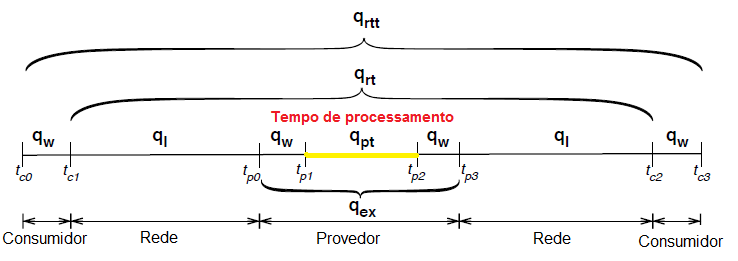
\includegraphics[width=1.0\textwidth]{ServiceInvocationTimes_1.png}
%              \caption{Instantes de tempo na utilização de um serviço Web}
%              %\label{fig:QoST_SLA_Mapping_Transformation}
%          \end{figure}	
%      }

%      \only<3>{	
%          \begin{figure}[!h]
%              \centering
%              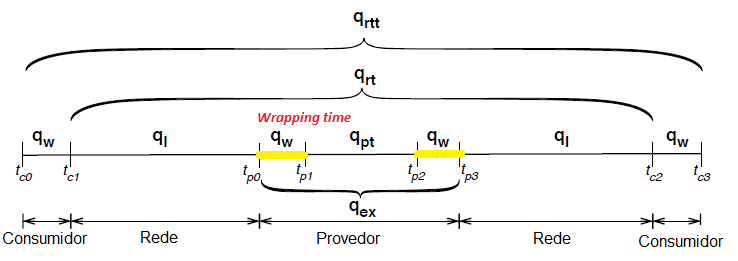
\includegraphics[width=1.0\textwidth]{ServiceInvocationTimes_2.png}
%              \caption{Instantes de tempo na utilização de um serviço Web}
%              %\label{fig:QoST_SLA_Mapping_Transformation}
%          \end{figure}	
%      }

 %      \only<4>{	
 %         \begin{figure}[!h]
 %             \centering
 %             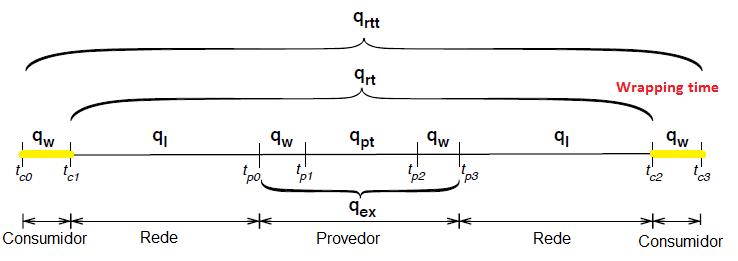
\includegraphics[width=1.0\textwidth]{ServiceInvocationTimes_2b.png}
 %             \caption{Instantes de tempo na utilização de um serviço Web}
 %             %\label{fig:QoST_SLA_Mapping_Transformation}
 %         \end{figure}	
 %     }

      \only<2>{	
          \begin{figure}[!h]
              \centering
              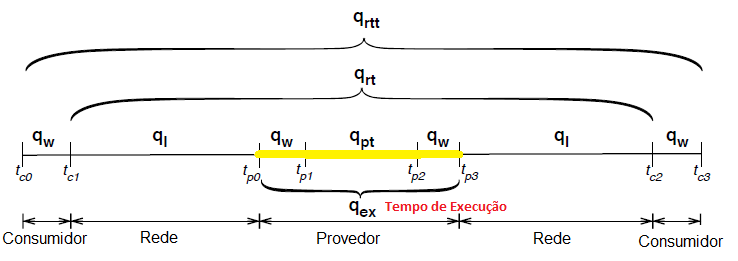
\includegraphics[width=1.0\textwidth]{ServiceInvocationTimes_3.png}
              \caption{Instantes de tempo na utilização de um serviço Web}
              %\label{fig:QoST_SLA_Mapping_Transformation}
          \end{figure}	
      }

      \only<3>{	
          \begin{figure}[!h]
              \centering
              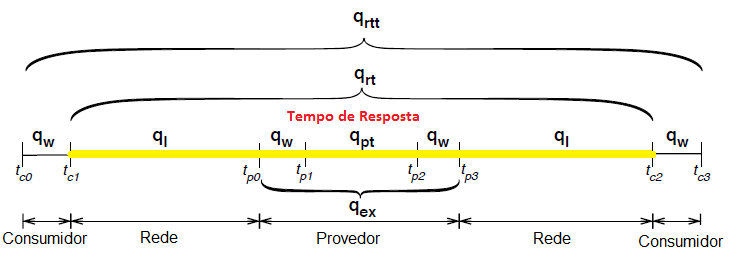
\includegraphics[width=1.0\textwidth]{ServiceInvocationTimes_5.png}
              \caption{Instantes de tempo na utilização de um serviço Web}
              %\label{fig:QoST_SLA_Mapping_Transformation}
          \end{figure}	
      }


      \only<4>{	
          \begin{figure}[!h]
              \centering
              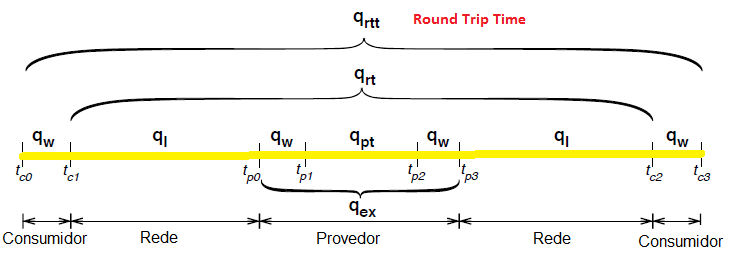
\includegraphics[width=1.0\textwidth]{ServiceInvocationTimes_6.png}
              \caption{Instantes de tempo na utilização de um serviço Web}
              %\label{fig:QoST_SLA_Mapping_Transformation}
          \end{figure}	
      }

    \end{frame}

    %-------------SLA ---------------%
    \begin{frame}{SLA }
        \begin{itemize}
          \item <1-> \textbf{Contrato} = Acordo formal entre uma ou mais partes, define requisitos e garantias das partes.
          \item <2-> \textbf{SLA} = Contrato que envolve requisitos e garantias de QoS.
          \item <3-> \textbf{Um SLA consiste de}:
            \begin{itemize}
              \item Partes
              \item Operações do serviço:
                    \begin{itemize}
                      \item <4-> Operações
                      \item <5-> \textbf{Parâmetros de SLA}: define as métricas de QoS envolvidas.
                    \end{itemize}
              \item Obrigações:
                      \begin{itemize}
                        \item <6-> \textbf{Garantias de QoS (objetivos ou restrições).}
                        \item <7-> Ações a serem tomadas se as garantias forem descumpridas (\textbf{reação}).
                      \end{itemize}
            \end{itemize}
            %\item <7-> Padrões: \textbf{WSLA}, WS-Agreement, WSOL, entre outros.
        \end{itemize}
        %\begin{block}{}\vspace{-.3\baselineskip}
         %{\Large SLA (Acordo de Nível de Serviço)}
        %\end{block}
    \end{frame}

  %%SLA Example
   \begin{frame}{ Exemplo de SLA}
     \only<1>{	
          \begin{figure}[!h]
              \centering
              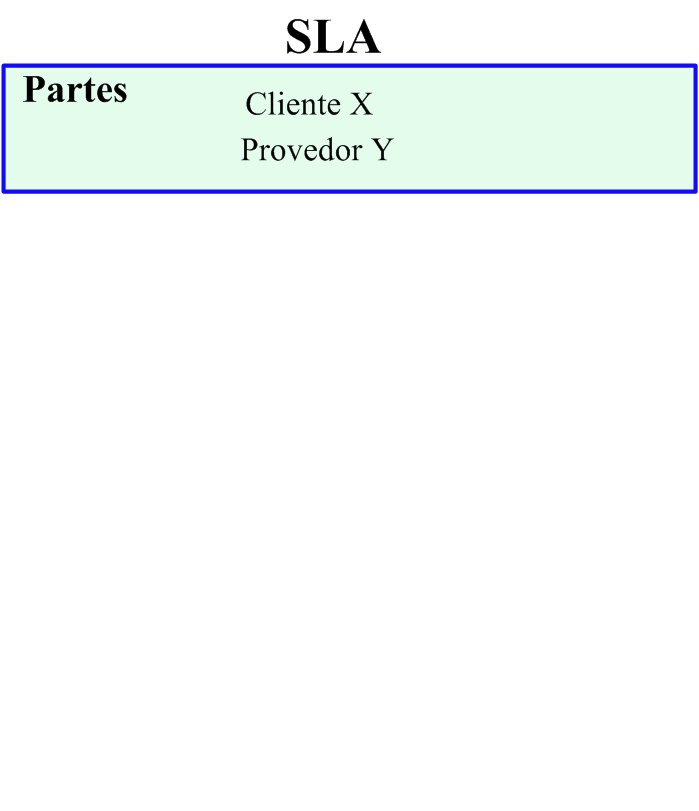
\includegraphics[width=0.5\textwidth]{SLAExample_1.png}
              \caption{Um exemplo simples de um SLA}
              %\label{fig:QoST_SLA_Mapping_Transformation}
          \end{figure}	
      }

      \only<2>{	
          \begin{figure}[!h]
              \centering
              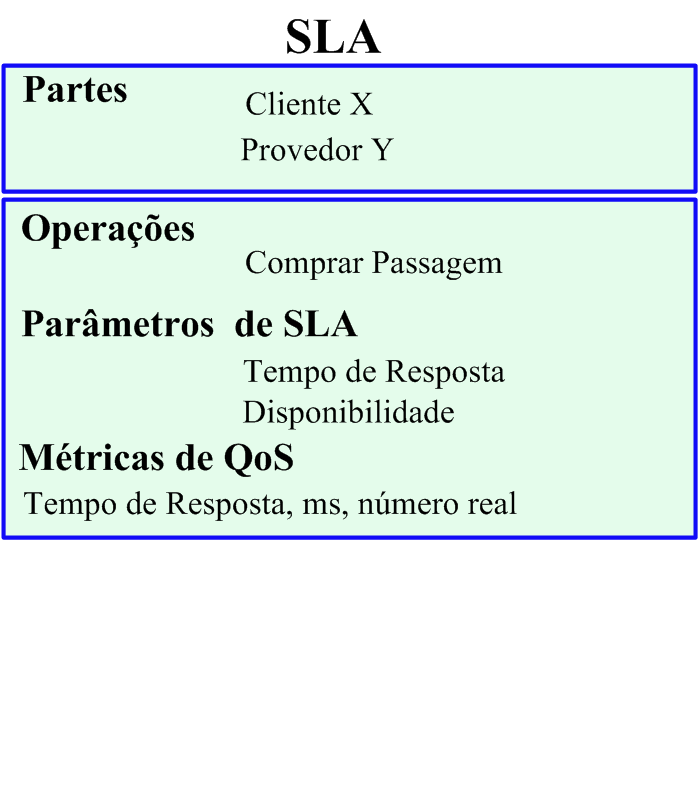
\includegraphics[width=0.5\textwidth]{SLAExample_2.png}
              \caption{Um exemplo simples de um SLA}
              %\label{fig:QoST_SLA_Mapping_Transformation}
          \end{figure}	
      }
      \only<3>{	
          \begin{figure}[!h]
              \centering
              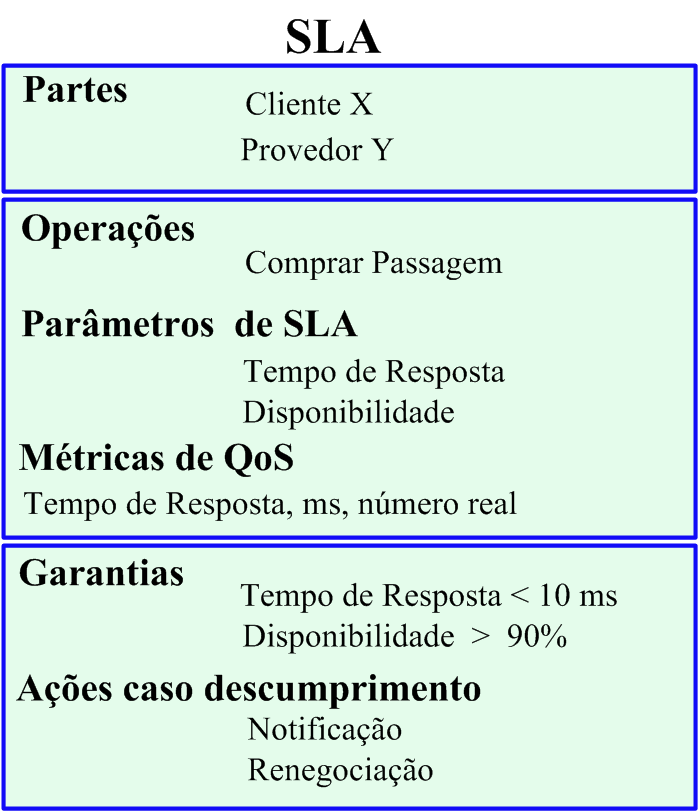
\includegraphics[width=0.5\textwidth]{SLAExample_3.png}
              \caption{Um exemplo simples de um SLA}
              %\label{fig:QoST_SLA_Mapping_Transformation}
          \end{figure}	
      }


   \end{frame}


  %%QoS Agregation
   \begin{frame}{Agregação de QoS}
        \begin{itemize}
          \item Processo de obter o valor cumulativo da QoS da composição a partir dos valores de QoS dos seus serviços
          componentes.
          \item Não existe solução geral.
          \item \colorbox{yellow}{Depende do atributo de QoS e do modelo de composição.}
          \item Abordagens:
          \begin{itemize}
            \item Somas, Máximos, Mínimos, Médias, etc.
            \item Analíticas: Redes de Petri, Redes de Fila, etc.
            \item Heurísticas: Algoritmos Genéticos.
            \item \textbf{Simulação}.
          \end{itemize}

        \end{itemize}
    \end{frame}

%%QoS Aggregation example
    \begin{frame}{Exemplo de Agregação de QoS}
      \begin{figure}[!h]
          \centering
          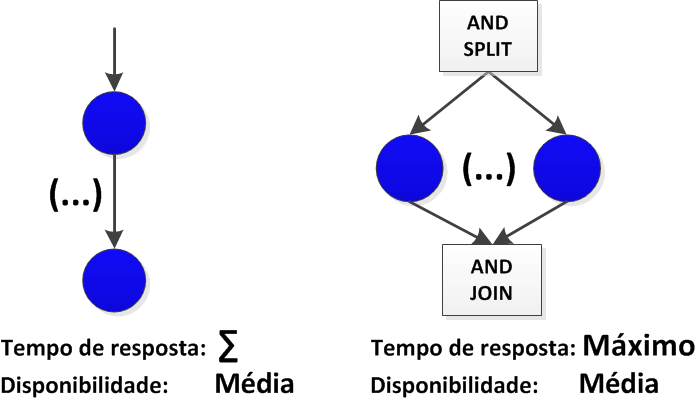
\includegraphics[width=0.6\textwidth]{WorkflowPatterns-QoS.png}
          \caption{Exemplo de Agregação de QoS}
          %\label{fig:QoST_SLA_Mapping_Transformation}
      \end{figure}	
    \end{frame}


% ------------------------------------------------------------------%
% ---------------- SLAs probabilísticos ----------------------------%
%\subsection{SLAs probabilísticos }
%--------------------------------------------------------
    \begin{frame}{Contratos Rígidos}
        \begin{itemize}
          \item <1-> Os contratos são tipicamente realizados em base a \textbf{restrições rígidas} (\emph{hard contracts}):
                \begin{itemize}
                  %\item <2->\colorbox{yellow}{Tempo de resposta $<$ 10 ms}
		  \item <2-> Tempo de resposta $<$ 10 ms.
                \end{itemize}
          \item <3->Contratos rígidos não refletem o comportamento dinâmico da QoS dos serviços Web.
        \end{itemize}
    \end{frame}


    \begin{frame}{Comportamento dinâmico de atributos de QoS}
      \begin{figure}[!h]
          \centering
          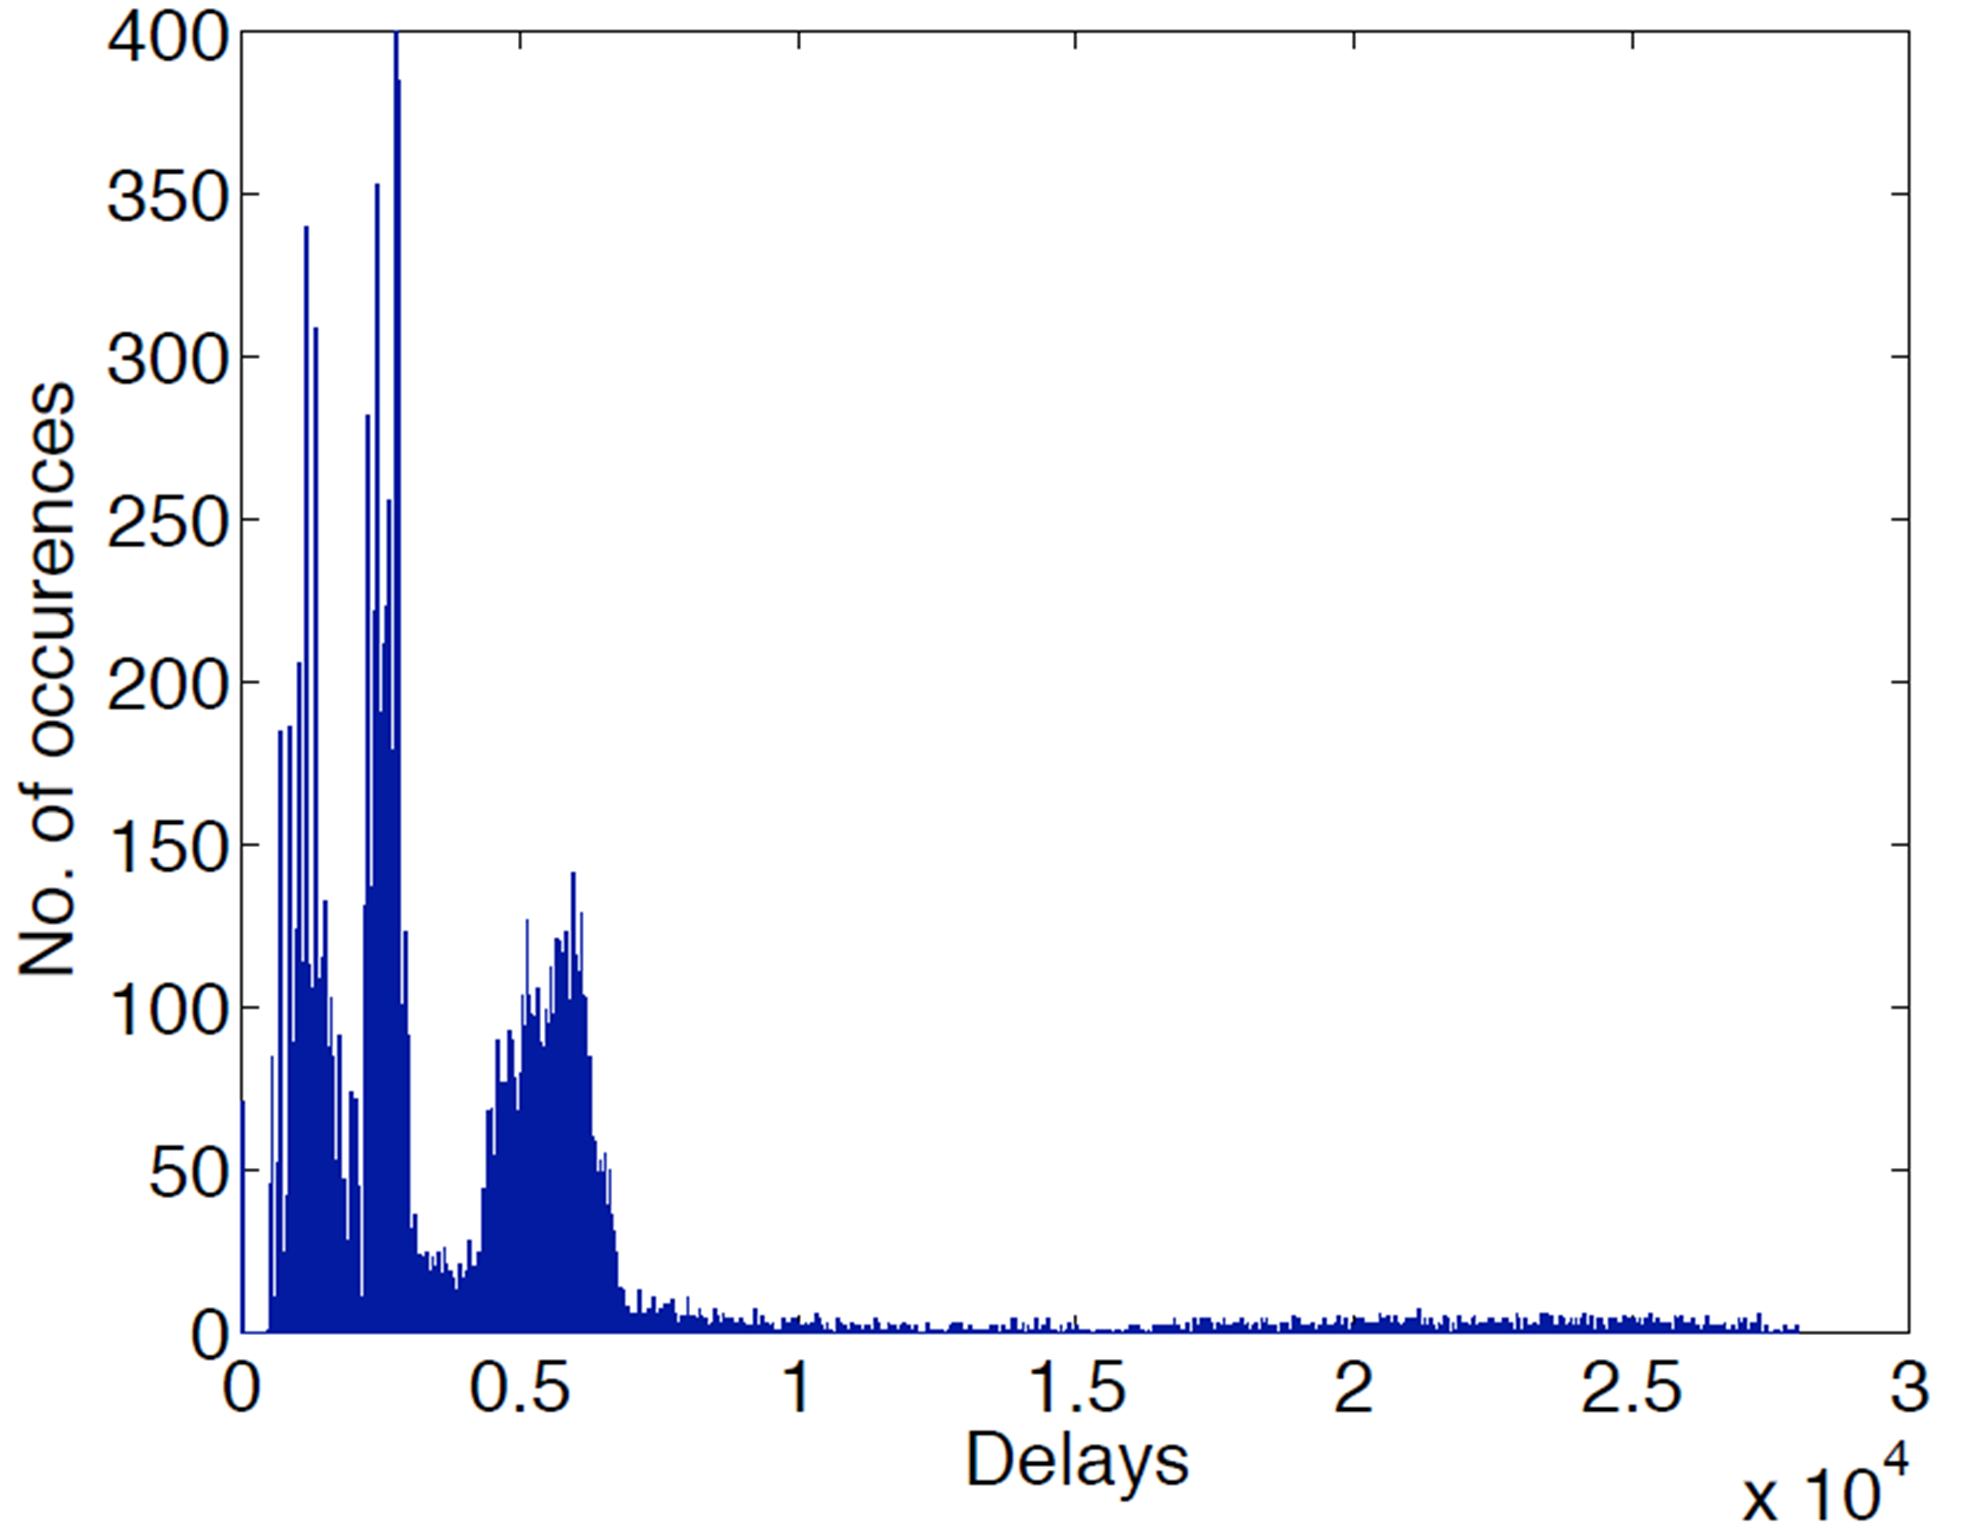
\includegraphics[width=0.6\textwidth]{hardContractsLimitations.png}
          \caption{Tempos de resposta de 20,000 chamadas de um serviço [Rosario et al., 2008] } %~\cite{Rosario2008}}
          %\label{fig:QoST_SLA_Mapping_Transformation}
      \end{figure}	

      \tiny{
        %\begin{thebibliography}{7}
         %         \beamertemplatearticlebibitems
         %   \bibitem[Rosario et al., 2008]{Rosario2008}
         %   Rosario S, Benveniste A, Haar S, Jard C. {\em Probabilistic QoS and Soft Contracts for Transaction-Based Web Services Orchestrations }. IEEE Transactions on Services Computing. 2008;1(4):187-200.
            %\newblock {\em {\tiny Probabilistic QoS and Soft Contracts for Transaction-Based Web Services Orchestrations }}.
            %\newblock {\tiny IEEE Transactions on Services Computing. 2008;1(4):187-200.}
        %\end{thebibliography}
      }
    \end{frame}

%---------------------------------------------------------------------------
    \begin{frame}{Contratos Não Rígidos}
        \begin{itemize}
          \item <1-> Contratos não rígidos ( \emph{soft contracts} ):
                \begin{itemize}
                  \item \textcolor{blue}{\textbf{Tempo de resposta $<$ 10 ms, em 95\% dos casos}}.
                \end{itemize}
                Desse jeito, não é possível compor esse tipo de restrições ou contratos, isto é,
                composição de restrições.
          \item <2-> \textbf{Solução:} contratos probabilísticos não rígidos (\emph{probabilistic soft contracts}).
                  \begin{itemize}
                  \item \textcolor{blue}{ \textbf{Para cada parâmetro de QoS (tempo de resposta). Eu ofereço sua distribuição de
                    probabilidade e garanto que não será pior do que isso}}.
                \end{itemize}
          \item <3-> As \textbf{restrições probabilísticas} podem ser compostas.
                \begin{itemize}
                  \item Existem algumas abordagens para orquestração.
                  \item \colorbox{yellow}{Não existem abordagens para coreografias}.
                  \item \colorbox{yellow}{Tratam somente tempo de resposta}.
                \end{itemize}
        \end{itemize}
    \end{frame}



%---- Definição de Contratos -------------------
%    \setbeamercovered{transparent}
%    \begin{frame}{Definição de Contratos}
%        \begin{itemize}
%          \item <1-> Na prática, as restrições ou contratos são definidos como um conjunto finito  de \textbf{quantis}  dos parâmetros de QoS.

%          \item <2-> Esses \textbf{quantis} definem uma distribuição empírica de probabilidade desses parâmetros de QoS.
%                \begin{itemize}
%                    \item <3->Por exemplo: %\textbf{quantis} de 25\%, 50\%, 90\%, 95\% e 98\% correspondem a tempos de %resposta máximos de 2.5ms, 4.5ms, 6.4ms, 13.8ms, e 23.5ms respectivamente.
%                        \begin{tabular}{|c|c|}
%                  \hline
                  % after \\: \hline or \cline{col1-col2} \cline{col3-col4} ...
%                  Quantis & Tempo de Resposta \\
%                  \hline
%                  25\% & 2.5 ms \\
%                  50\% & 4.5 ms \\
%                  90\% & 6.4 ms \\
%                  95\% & 13.8 ms \\
%                  98\% & 23.5 ms \\
%                  \hline
%                \end{tabular}
%                \end{itemize}

%          \item <4-> O conjunto de restrições ou contratos compõem um SLA.

          %\item <5->WSLA é o padrão para especificar SLAs.

%        \end{itemize}
%    \end{frame}



% ------------- Monitoramento baseado em QoS -----------------------%
% ------------------------------------------------------------------%
%\subsection{Monitoramento baseado em QoS }
    \begin{frame}{Monitoramento baseado em QoS}
	Responsabilidades:
        \begin{itemize}
          \item Mede e calcula valores de métricas de QoS, também inclui \textbf{ agregação} de valores dos atributos de QoS.
          \item Verifica se existe violação de alguma restrição de QoS.
          \item \colorbox{yellow}{ Monitoramento de Coreografias deve ser ``não intrusivo''}.
          %\item Outras responsabilidades.
        \end{itemize}
    \end{frame}

%----- Abordagens de Monitoramento  -----------------------------------
    \begin{frame}{Abordagens de Monitoramento }
	\only<1>{	
	  Monitoramento Intrusivo: \textbf{Instrumentação}
          \begin{figure}[!h]
              \centering
              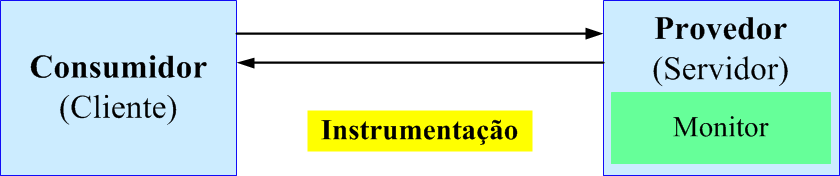
\includegraphics[width=0.8\textwidth]{MonitoringApproaches_1.png}
              \caption{Monitoramento por Instrumentação}
              %\label{fig:QoST_SLA_Mapping_Transformation}
          \end{figure}	
        }

        \only<2>{	
	  Monitoramento Não Intrusivo: \textbf{Interceptação}
          \begin{figure}[!h]
              \centering
              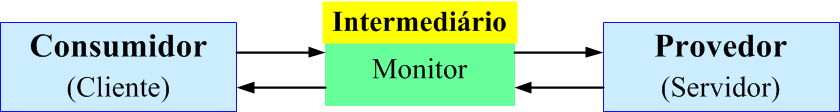
\includegraphics[width=0.8\textwidth]{MonitoringApproaches_2.png}
              \caption{Monitoramento por Interceptação}
              %\label{fig:QoST_SLA_Mapping_Transformation}
          \end{figure}	
        }

        \only<3>{	
	  Monitoramento Não Intrusivo: \textbf{\textit{Probe-Request}}
          \begin{figure}[!h]
              \centering
              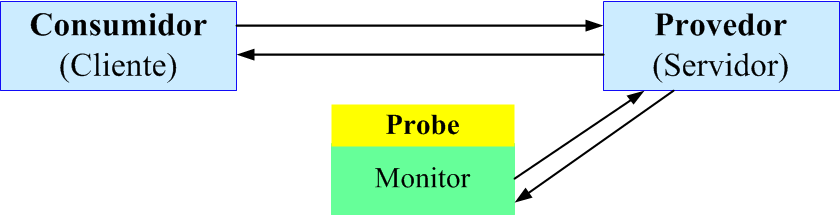
\includegraphics[width=0.8\textwidth]{MonitoringApproaches_3.png}
              \caption{Monitoramento mediante Probe-Request}
              %\label{fig:QoST_SLA_Mapping_Transformation}
          \end{figure}	
        }

        \only<4>{	
	  Monitoramento Não Intrusivo: \textbf{\textit{Sniffing}}
          \begin{figure}[!h]
              \centering
              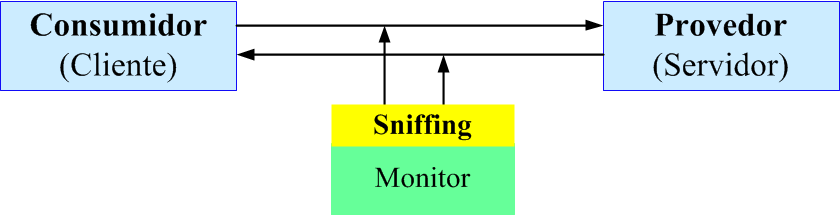
\includegraphics[width=0.8\textwidth]{MonitoringApproaches_4.png}
              \caption{Monitoramento mediante sniffing}
              %\label{fig:QoST_SLA_Mapping_Transformation}
          \end{figure}	
        }

    \end{frame}


  % ---- Monitoramento e Adaptação %
%  \begin{frame} {Monitoramento e Adaptação}
%      \only<1>{	
%          \begin{figure}[!h]
%              \centering
%              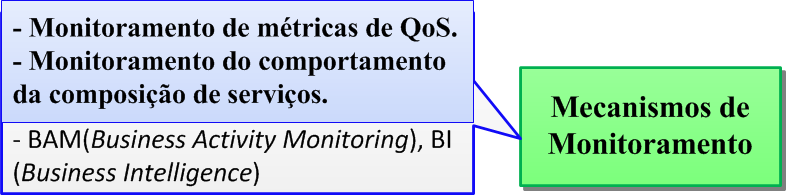
\includegraphics[width=0.7\textwidth]{ConceptualingMonitoringAdaptation_1.png}
%              \caption{Monitoramento e Adaptação}
              %\label{fig:QoST_SLA_Mapping_Transformation}
%          \end{figure}	
%        }
%  \end{frame}

  % ---- Monitoramento e Adaptação %
  \begin{frame} {Camadas no Monitoramento }
      \only<1>{	
          \begin{figure}[!h]
              \centering
              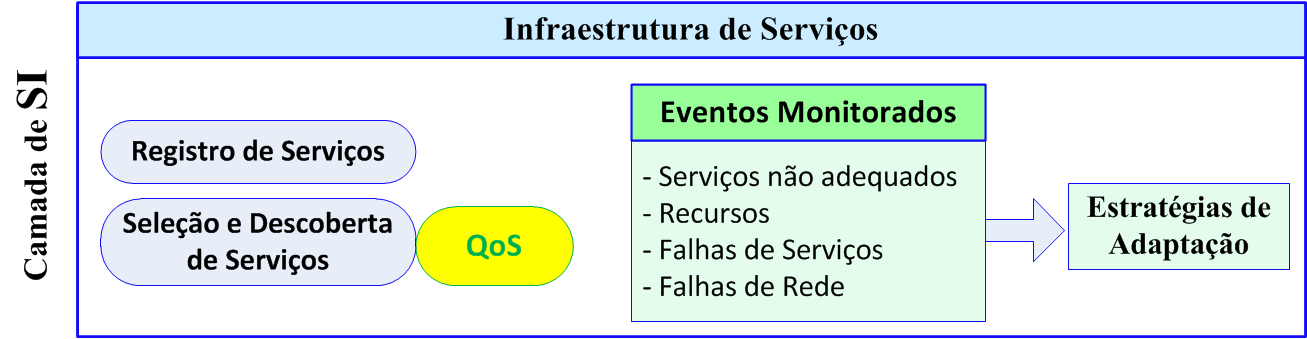
\includegraphics[width=0.8\textwidth]{MonitoringLayers_1.png}
              \caption{Camadas do Monitoramento}
              %\label{fig:QoST_SLA_Mapping_Transformation}
          \end{figure}	
        }
      \only<2>{	
          \begin{figure}[!h]
              \centering
              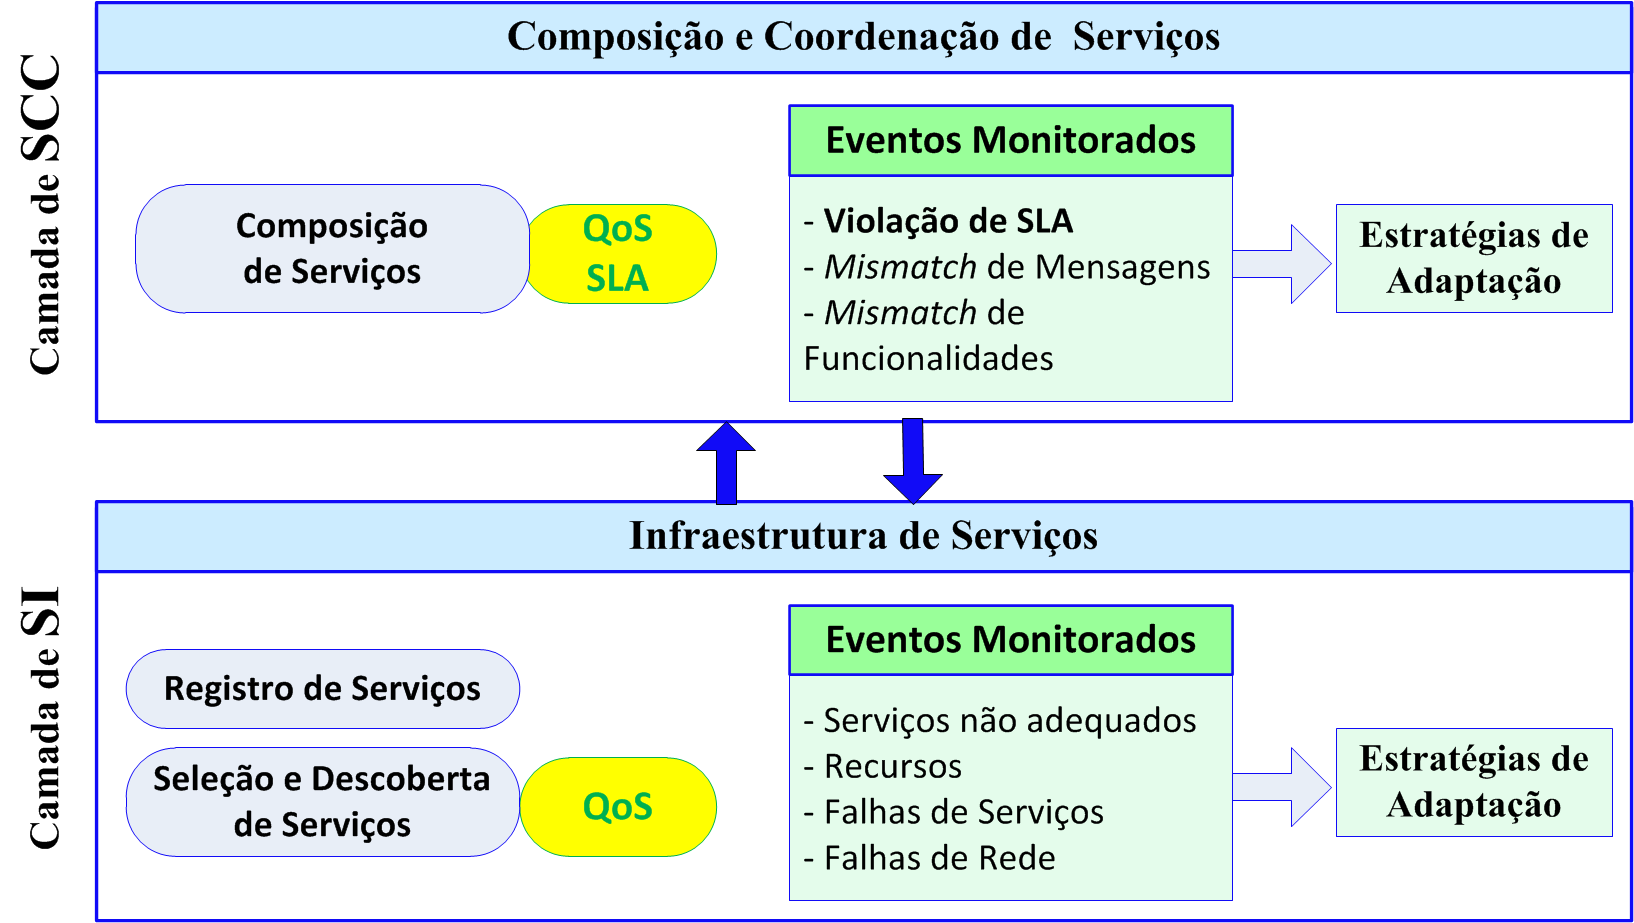
\includegraphics[width=0.85\textwidth]{MonitoringLayers_2.png}
              \caption{Camadas do Monitoramento}
              %\label{fig:QoST_SLA_Mapping_Transformation}
          \end{figure}	
        }
      \only<3>{	
          \begin{figure}[!h]
              \centering
              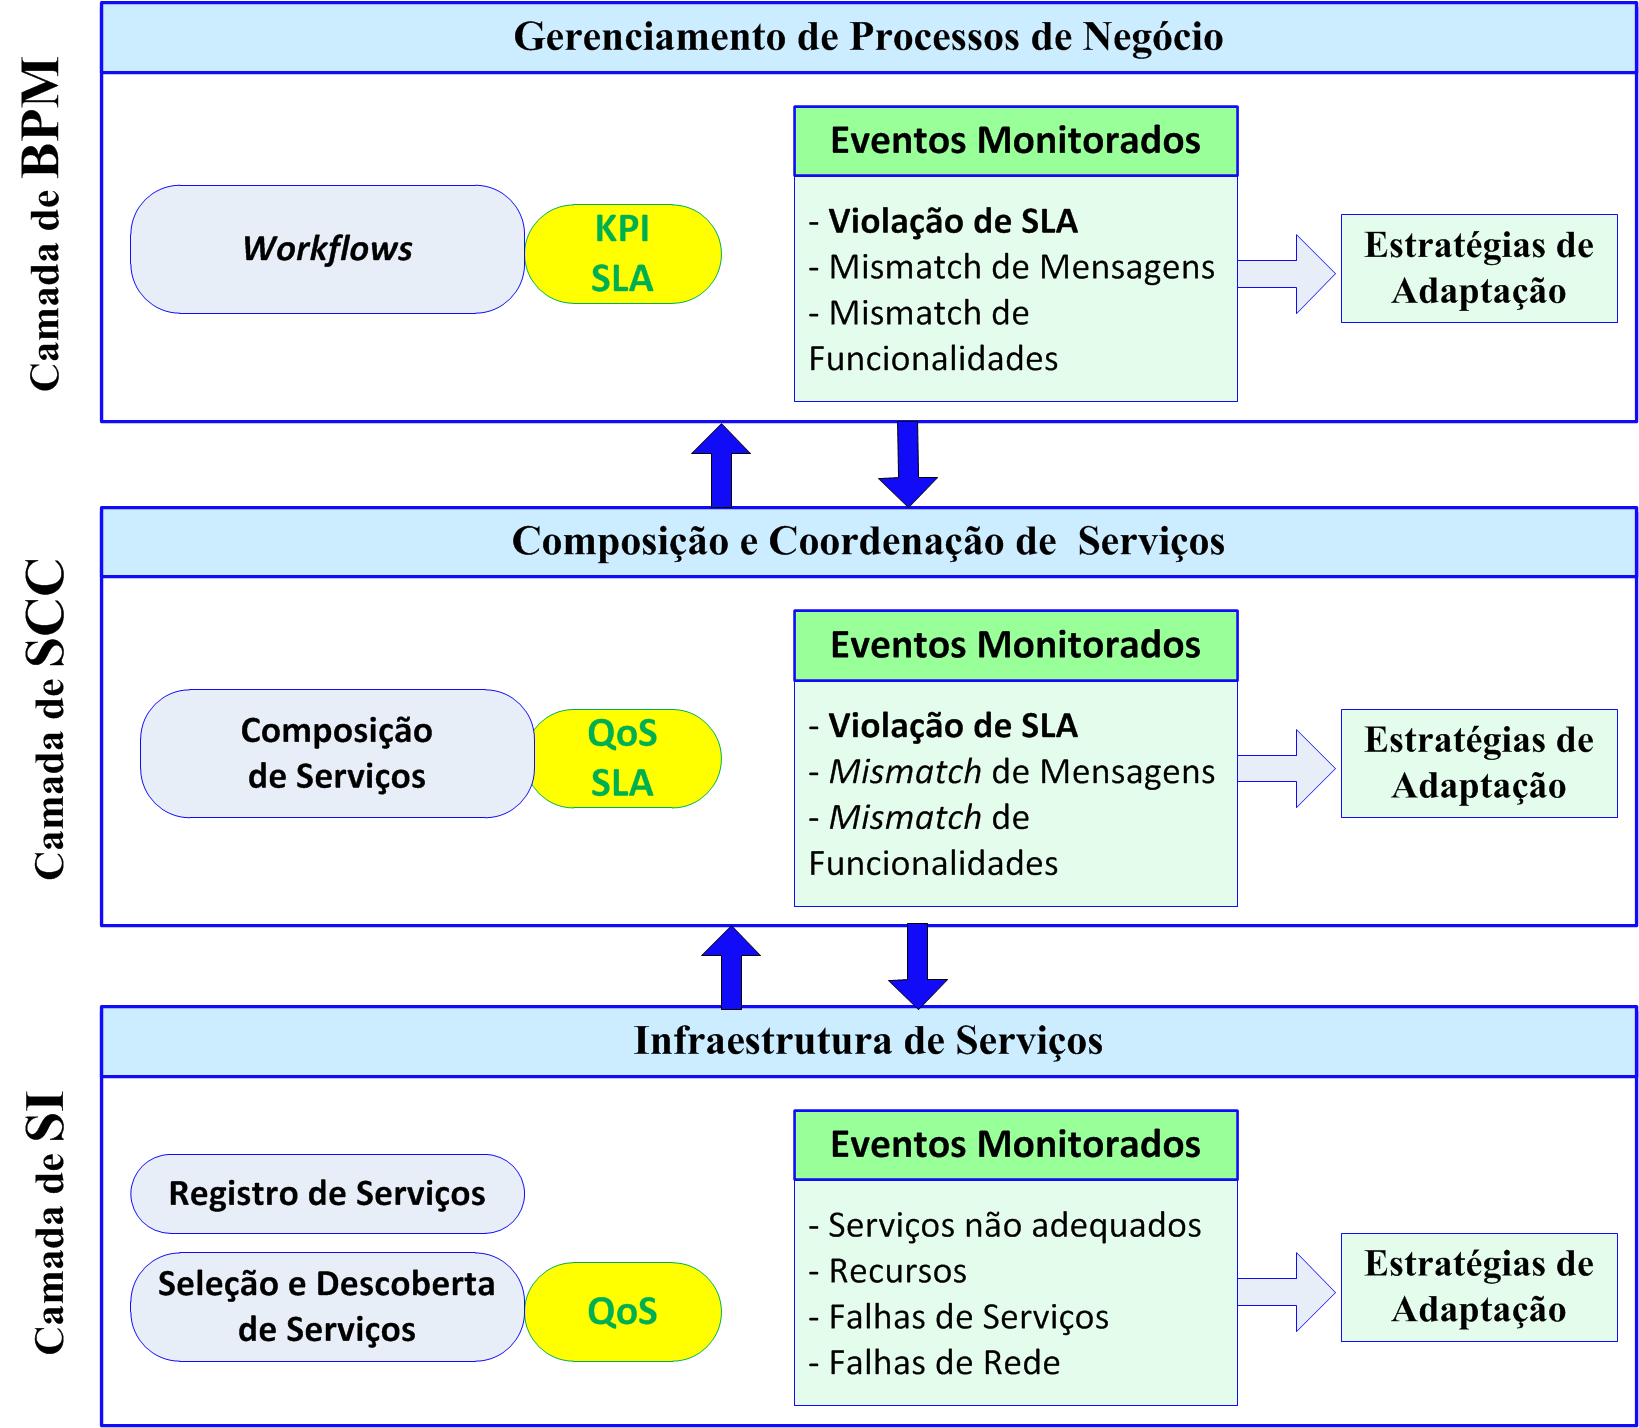
\includegraphics[width=0.8\textwidth]{MonitoringLayers_3.png}
              \caption{Camadas do Monitoramento}
              %\label{fig:QoST_SLA_Mapping_Transformation}
          \end{figure}	
        }
      \only<4>{	
          \begin{figure}[!h]
              \centering
              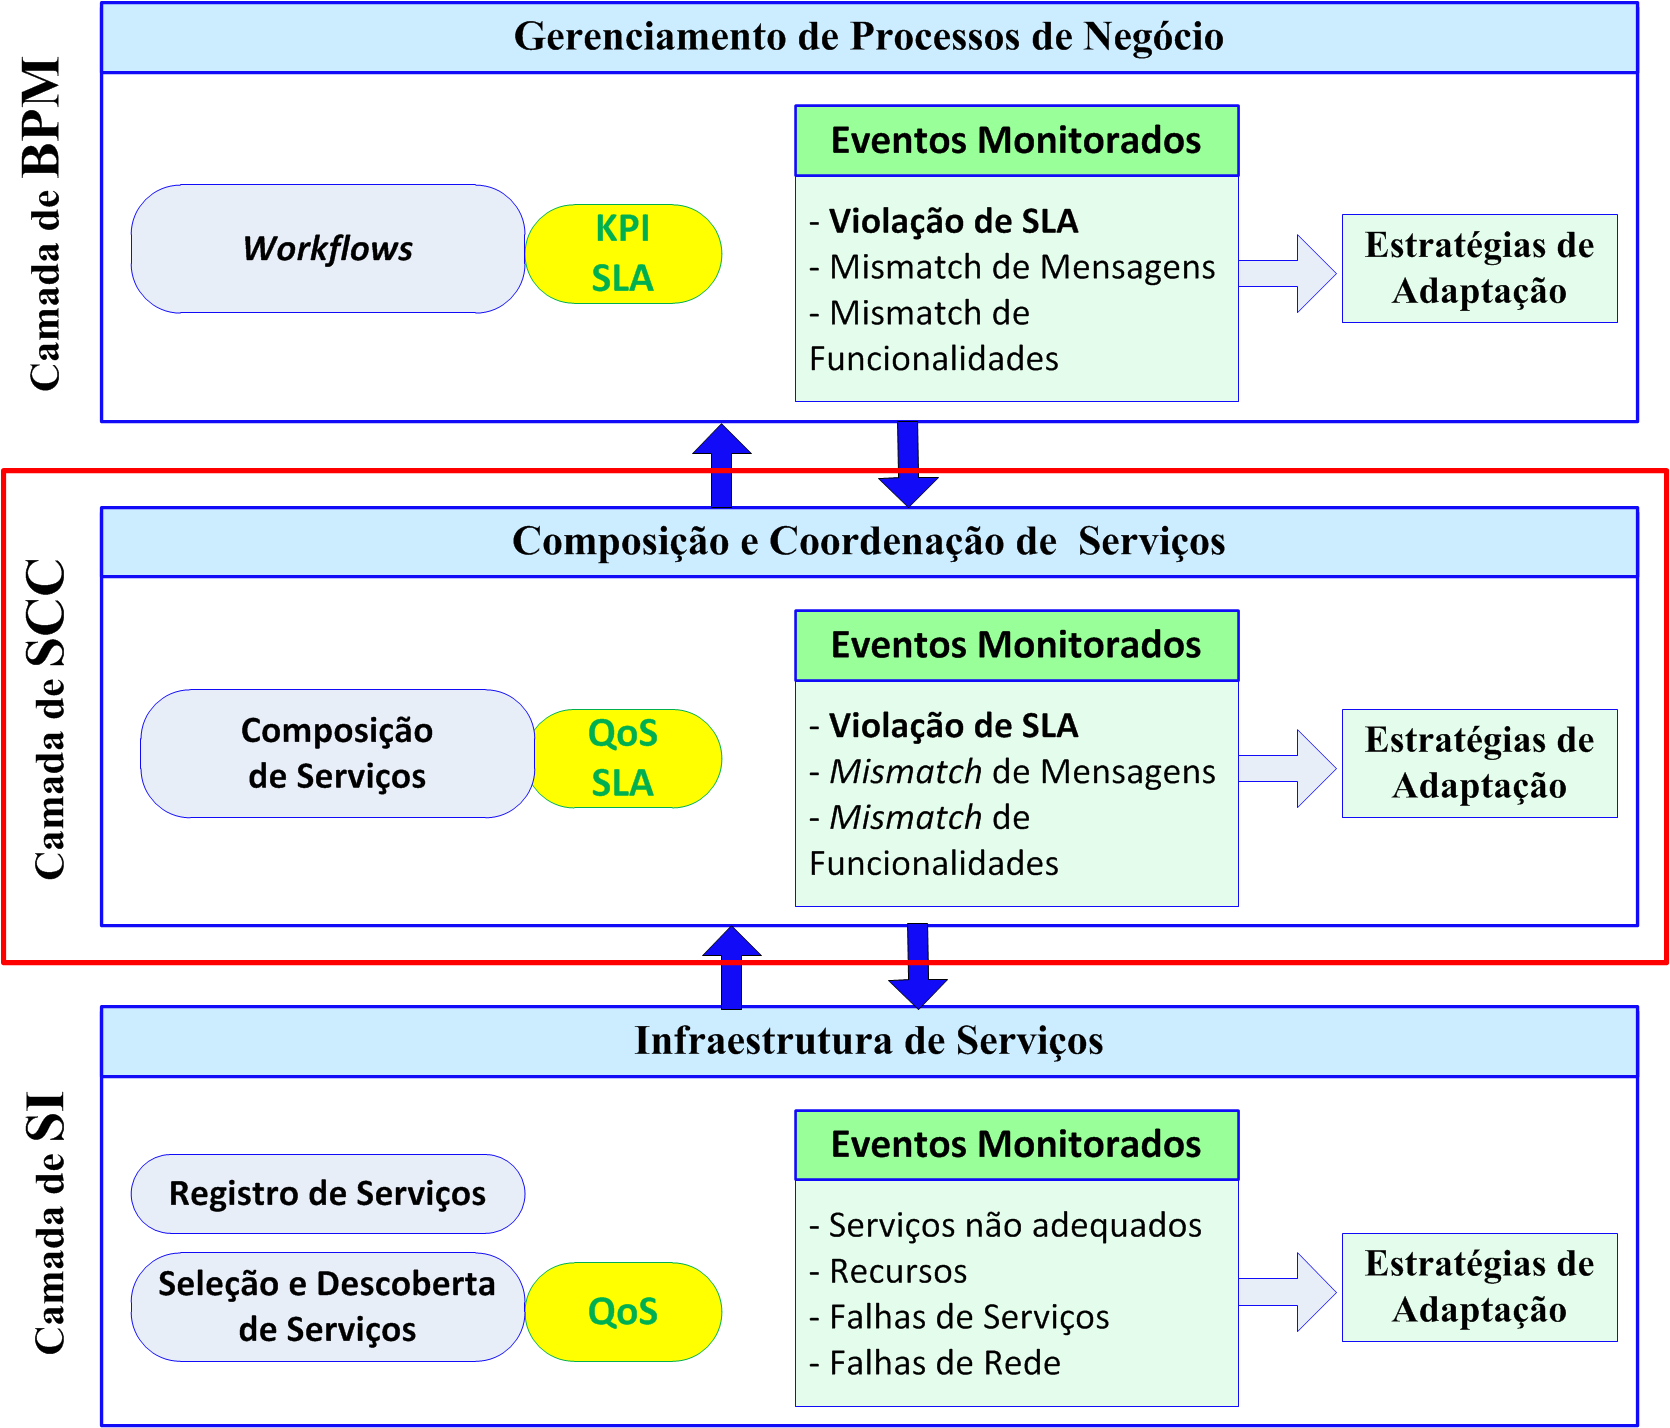
\includegraphics[width=0.8\textwidth]{MonitoringLayers_4.png}
              \caption{Camadas do Monitoramento}
              %\label{fig:QoST_SLA_Mapping_Transformation}
          \end{figure}	
        }
  \end{frame}


  %--  QoS e SLA Multi-camada%
  \begin{frame} {QoS multi-camada em coreografias de serviços Web}
          \begin{figure}[!h]
              \centering
              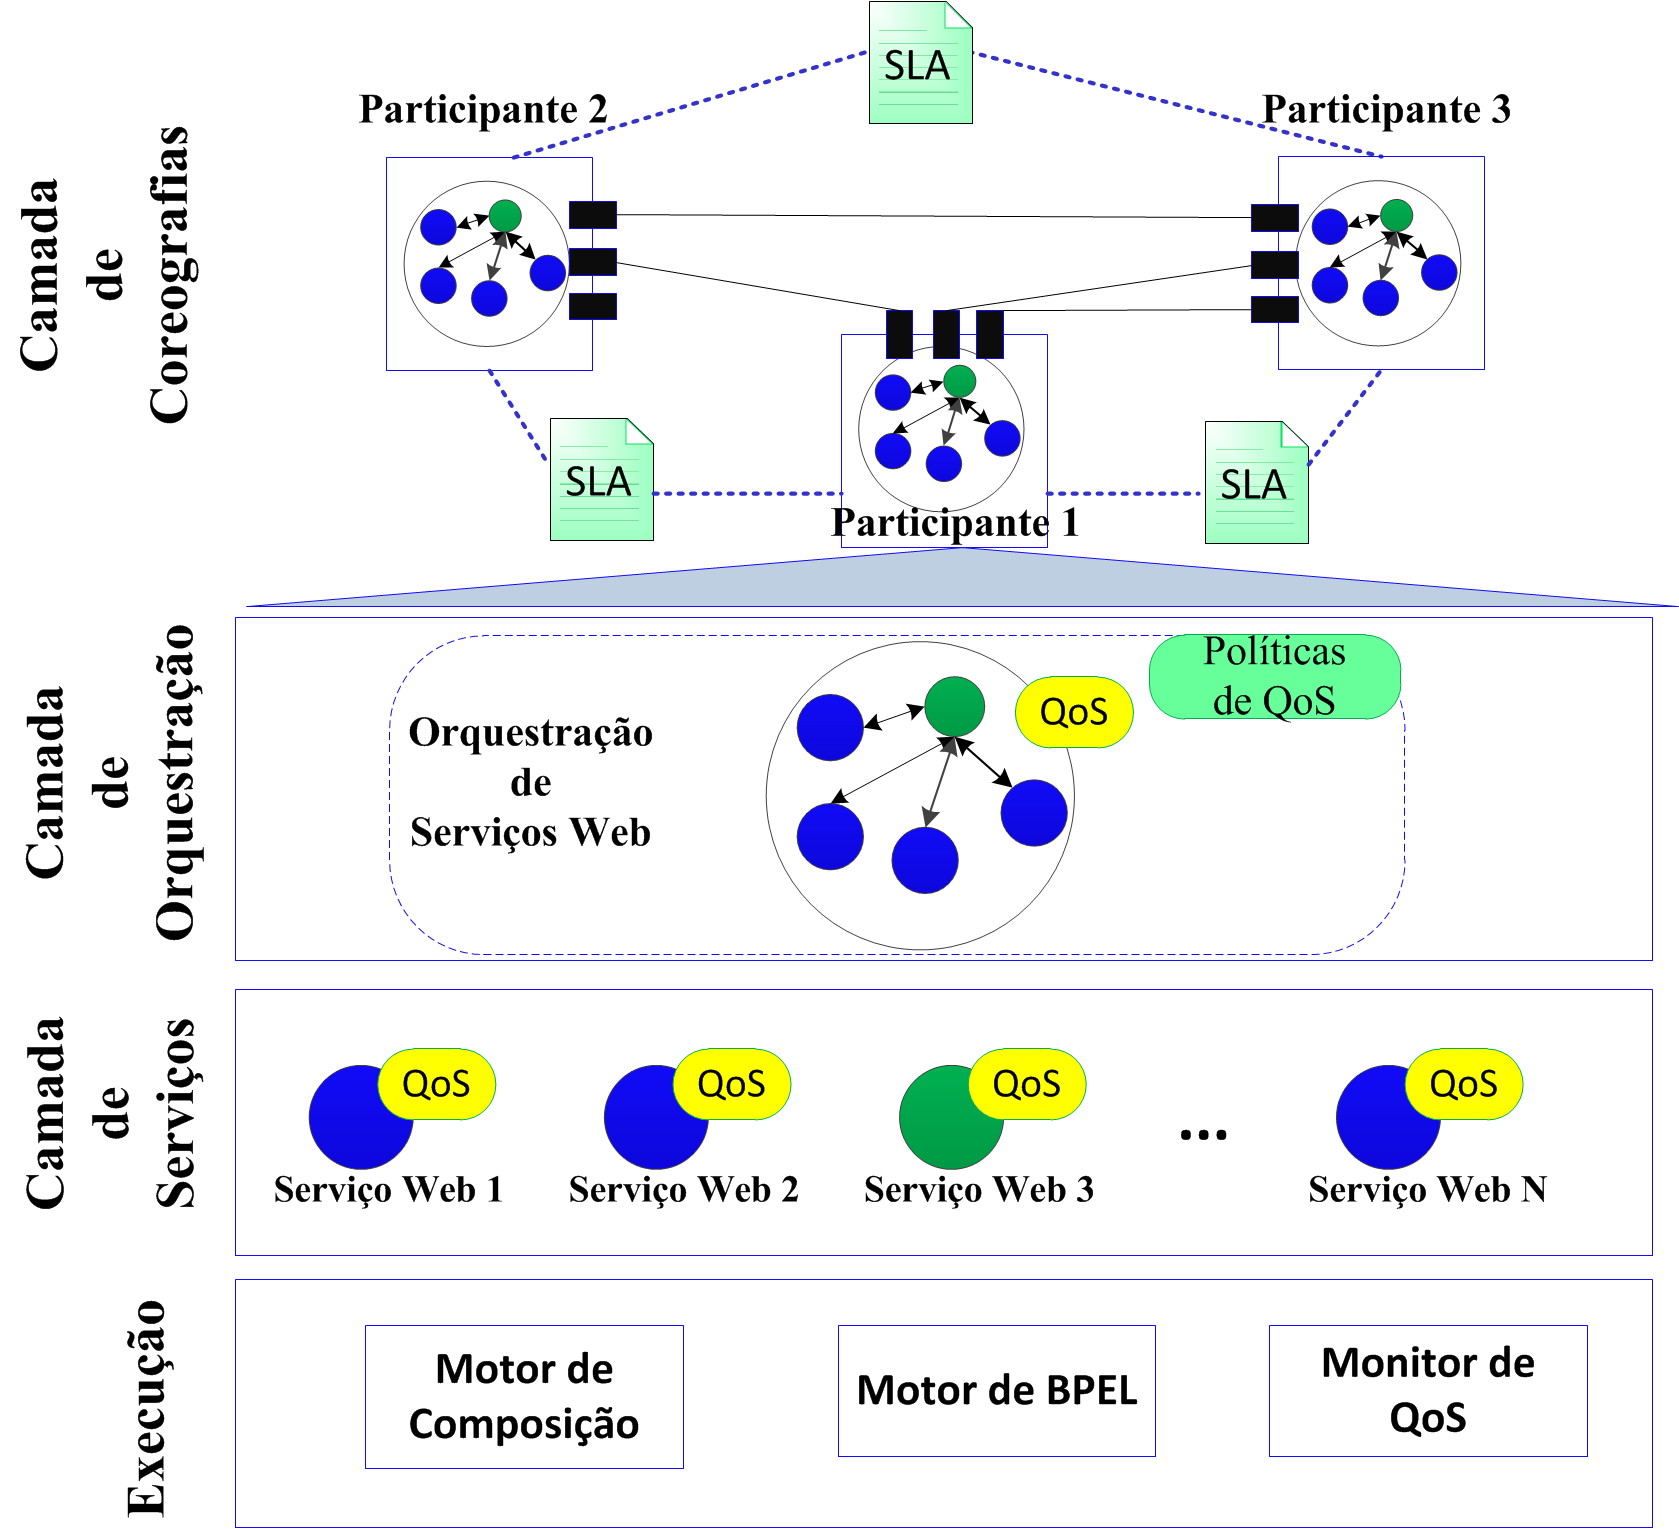
\includegraphics[width=0.65\textwidth]{./figures/Choreography-MultiTier.png}
              \caption{Integração de QoS e SLA multi-camada em coreografias } %(baseado em [[Rosenberg et al., 2009]])}
              %\label{fig:QoST_SLA_Mapping_Transformation}
          \end{figure}	
  \end{frame}



% ------------------------------------------------------------------%
% ------------- Trabalhos Relacionados -----------------------%
% ------------------------------------------------------------------%
\section{Trabalhos Relacionados}
%QoS
%Monitoramento
  \begin{frame}{ Monitoramento de Coreografias de Serviços Web Baseado em QoS }

      \begin{itemize}
	\item <1-> \small{ (Xiangpeng et al.,2007), (Pandey and Chaudhary, 2008) e (Pandey, 2010)} :
	 \begin{itemize}
	    \item Métodos formais para especificar QoS em coreografias.
	    \item \color{red} {Focado somente na linguagem}.
	 \end{itemize}
	\item <2-> \small{ (Wetzstein et al., 2010)}:
	    \begin{itemize}
	      \item Monitoramento de processos inter-organizacionais.
	      \item \color{red} {Foco em KPIs e não em QoS}.
	    \end{itemize}
      %\end{itemize}
  %\end{frame}


  %\begin{frame}{ Monitoramento de Coreografias de Serviços Web Baseado em QoS (2/2)}
   %   \begin{itemize}
	\item <3-> \small{ (Ul Haq et al., 2010) }:
	    \begin{itemize}
	      \item Agregações hierárquicas de SLAs em coreografias.
	      \item Framework baseado em regras.
	      \item \color{red}{Foco em processos de negócio e KPIs}.
	    \end{itemize}
	\item <4-> \small{ (Xia et al., 2009) }:
	    \begin{itemize}
	      \item Predição analítica de QoS em coreografias em \color{red}{WSCI}. %\footnote{Redes de Petri Generalizadas}.
	      \item \color{red}{Foco na linguagem}.
	      %\item \color{Teórico e não trata SLAs}.
	    \end{itemize}
	\item <5-> \small{ (Rosenberg, 2009) }:
	    \begin{itemize}
	      \item Modelo multi-camada  de QoS para coreografias de serviços Web.
	      \item \color{red}{Sem uma técnica para estabelecer SLAs}.
          \item \color{red}{Foco em restrições rígidas}.
	    \end{itemize}
      \end{itemize}

   \end{frame}

  \begin{frame}{ Monitoramento de Serviços Usando SLAs Probabilísticos}
      \begin{itemize}
	\item <1-> (Rosario et al., 2008) e (Rosario et al., 2009)
	    \begin{itemize}
	      \item Método de Monte-Carlo para definir SLAs em orquestrações.
	      \item \color{red}{Foco no tempo de resposta}.
	      \item Monitoramento de SLAs probabilísticos em \color{red}{orquestrações} de serviços usando \color{red}{Orc}.
	      %\item Não está baseada em eventos e não possui uma implementação com motores BPEL.
	    \end{itemize}
	
	\item <2-> (Zheng et al., 2010):
	    \begin{itemize}
	      \item A Função Densidade de Probabilidade (PDF) da QoS. %de um serviço Web é mais adequada e melhor do que outras.
	      \item Demonstrações por meio de simulações.
	      \item \color{red}{Foco no tempo de resposta e não trata SLAs}.
	    \end{itemize}
      \end{itemize}

   \end{frame}


%  \begin{frame}{ Simulador de Coreografias de Serviços Web}
%      \begin{itemize}
%	\item <1-> WS-CDL+ (Rosario et al., 2008) e (Rosario et al., 2009)
%	    \begin{itemize}
%	      \item motor de execução de coreografias para WS-CDL.
%	      \item \color{red}{É apenas um protótipo}.
%	    \end{itemize}
%	
%	\item <2-> (Zheng et al., 2010):
%	    \begin{itemize}
%	      \item A Função Densidade de Probabilidade (PDF) da QoS. %de um serviço Web é mais adequada e melhor do que outras.
%	      \item Demonstrações por meio de simulações.
%	      \item \color{red}{Foco no tempo de resposta e não trata SLAs}.
%	    \end{itemize}
 %     \end{itemize}

  % \end{frame}




% ------------------------------------------------------------------%
% -------------        PROPOSTA    ---------------------------------%
% ------------------------------------------------------------------%
\section{Proposta}
%\section{Metodologia}

\subsection{Visão Geral}
%---------- Proposta ----------------
   \begin{frame}{Contribuições}

      \begin{itemize}
	  \item <1->  Desenvolvimento de um simulador de coreografias com suporte de QoS.
          \item <2-> Mecanismos para definir requisitos de QoS em coreografias de serviços Web. Para tanto utilizaram-se duas abordagens:
             \begin{itemize}
                  \item \textbf{Analítica}:  Usando Redes de Petri Estocásticas Generalizadas (GSPN) como representação intermediária
		    da especificação de uma coreografia.
                  \item \textbf{Simulações}: Por meio de avaliações de desempenho e modelos de falha usando o simulador de coreografias.
                  %\item Parâmetros envolvidos: número de quantis, qual distribuição de probabilidade, tamanho da zona de tolerância, entre outros.
            \end{itemize}

         \item <3-> Definição de restrições  probabilísticas de QoS entre os serviços de uma  coreografia de serviços Web.
	 \item <4-> Proposta de um mecanismo de monitoramento de coreografias para detectar violações de SLA com restrições de QoS probabilísticas.
	 \item <5->\textbf{Atributos de QoS}: tempo de resposta, tempo de processamento, largura de banda e latência de rede.
         %\item Atributos de QoS: tempo de resposta, latência de rede e largura de banda (monitoramento passivo).
         %\item <5->Implementação do monitoramento.
       \end{itemize}


   \end{frame}



  \begin{frame}{Etapas}
    %\begin{itemize}
    %  \item <1->\textbf{Estabelecimento de SLAs} probabilí­sticos para coreografias de serviços Web.
    %  \item <2->\textbf{Monitor não instrusivo} baseado em eventos para coreografias de serviços Web.
    %  \item <3->\textbf{Detecção de violações de SLAs probabilí­sticos}.
    %  \item <4->\textbf{Atributos de QoS}: tempo de resposta, largura de banda e atraso.
    %\end{itemize}
    \only<1>{	
		\begin{figure}
		\centering
		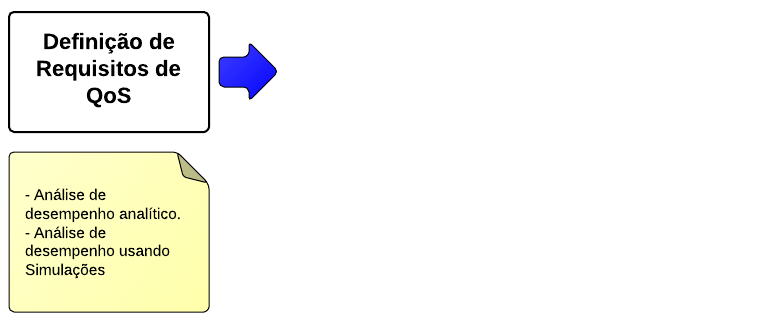
\includegraphics[width=1.0\textwidth]{MonitoringStages1.png}
		\caption{Etapas para atingir o monitoramento de coreografias}
		\end{figure}	
	}
    \only<2>{	
		\begin{figure}
		\centering
		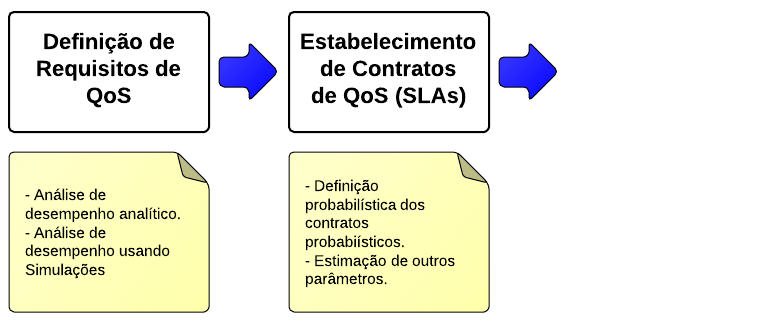
\includegraphics[width=1.0\textwidth]{MonitoringStages2.png}
		\caption{Etapas para atingir o monitoramento de coreografias}
		\end{figure}	
	}
    \only<3>{	
		\begin{figure}
		\centering
		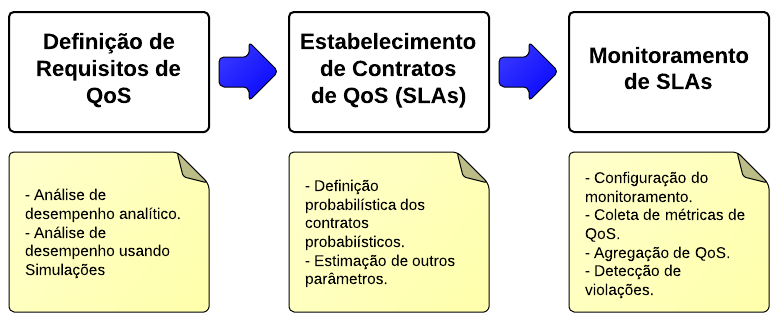
\includegraphics[width=1.0\textwidth]{MonitoringStages3.png}
		\caption{Etapas para atingir o monitoramento de coreografias}
		\end{figure}	
	}	
  \end{frame}

  \begin{frame}{Elementos BPMN 2 Suportados }
      \begin{figure}[!h]
	\centering
	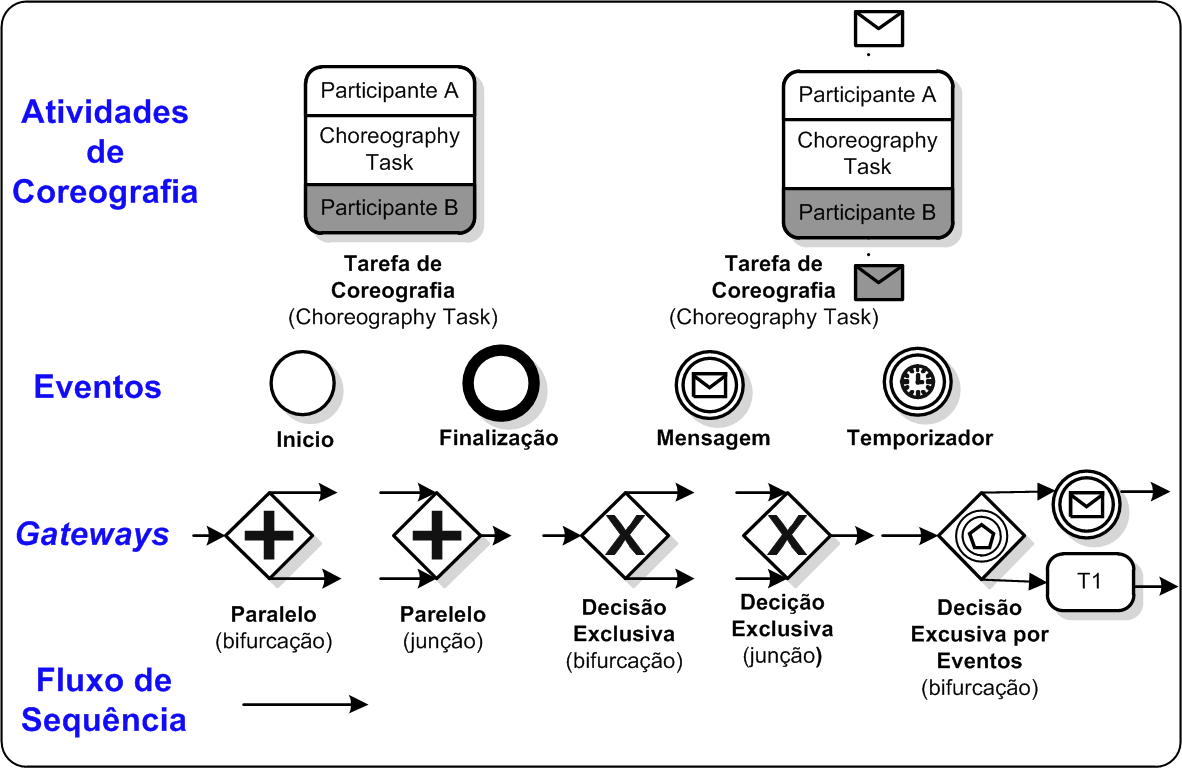
\includegraphics[width=0.7\textwidth]{./figures/BPMNBasicChoroegraphy.png}
	\caption{Elementos BPMN suportados.}
	\label{fig:ChoreographyElements}
    \end{figure}

  \end{frame}


%----- Monitoramento de Coreografias de Serviços -----------
    %\begin{frame}{Monitoramento de Coreografias de Serviços}
    \begin{frame}{Arquitetura do monitoramento para detectar violações de SLA}
    %\begin{picture}(0,0)(10,10)
    %	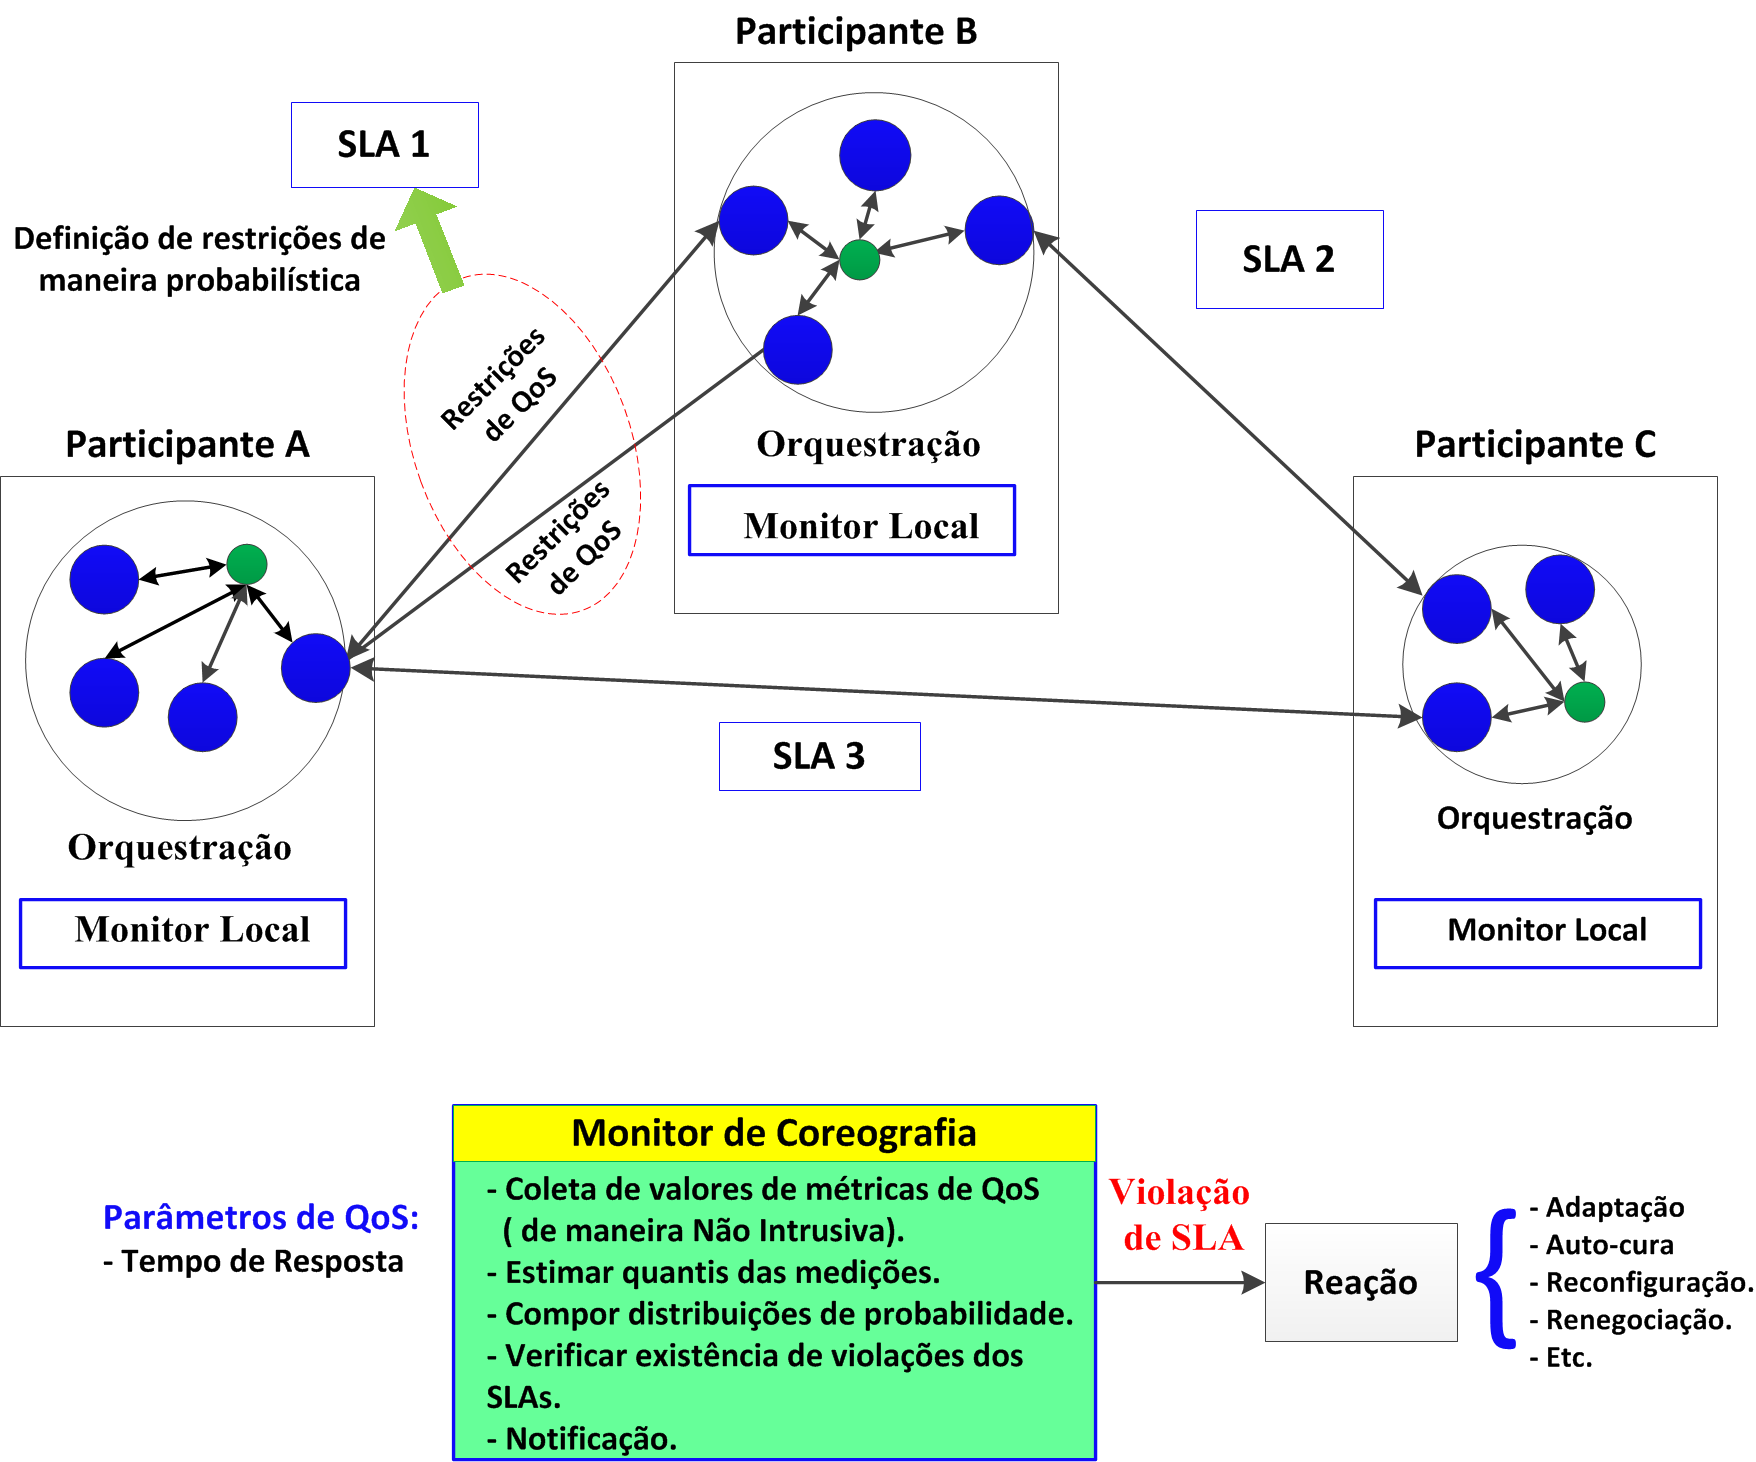
\includegraphics[width=110mm, height=90mm ]{MonitoringOverview.png}
    %\end{picture}
      \only<1>{	
          \begin{figure}
              \centering
              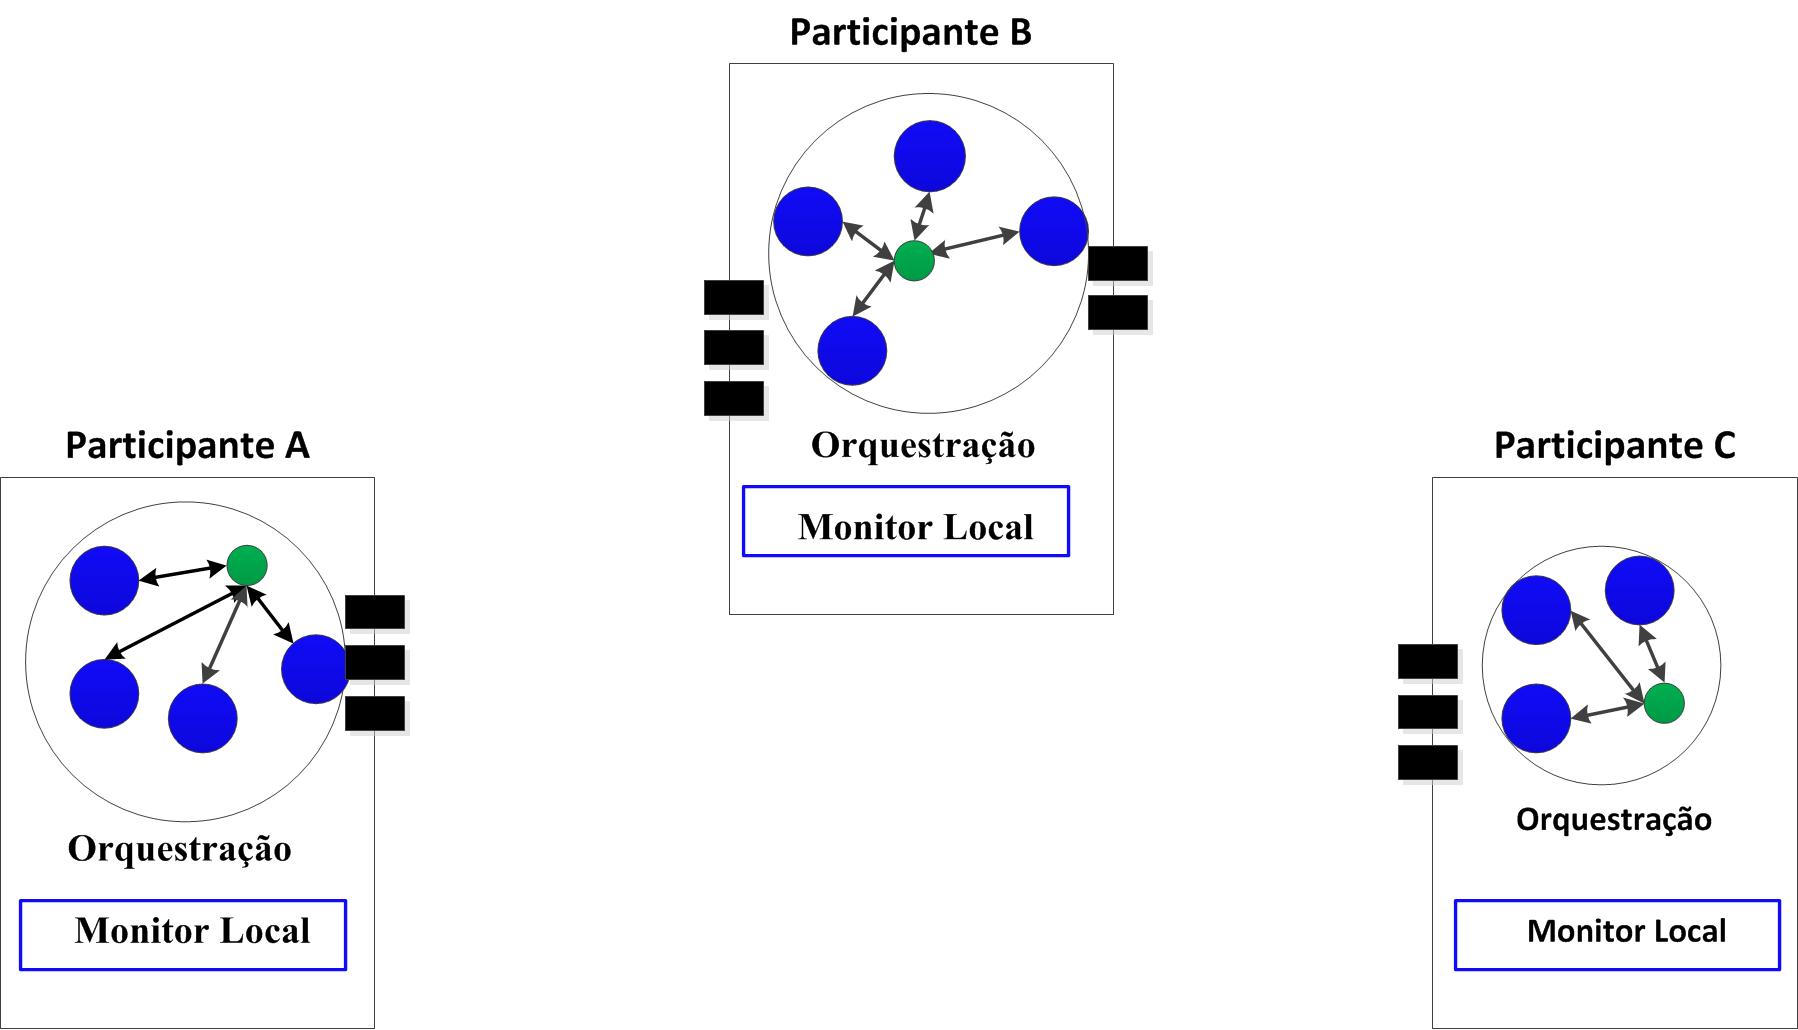
\includegraphics[width=0.9\textwidth]{MonitoringOverview_1.png}
              \caption{Perspectiva Geral do monitoramento proposto}
          \end{figure}	
      }

       \only<2>{	
          \begin{figure}
              \centering
              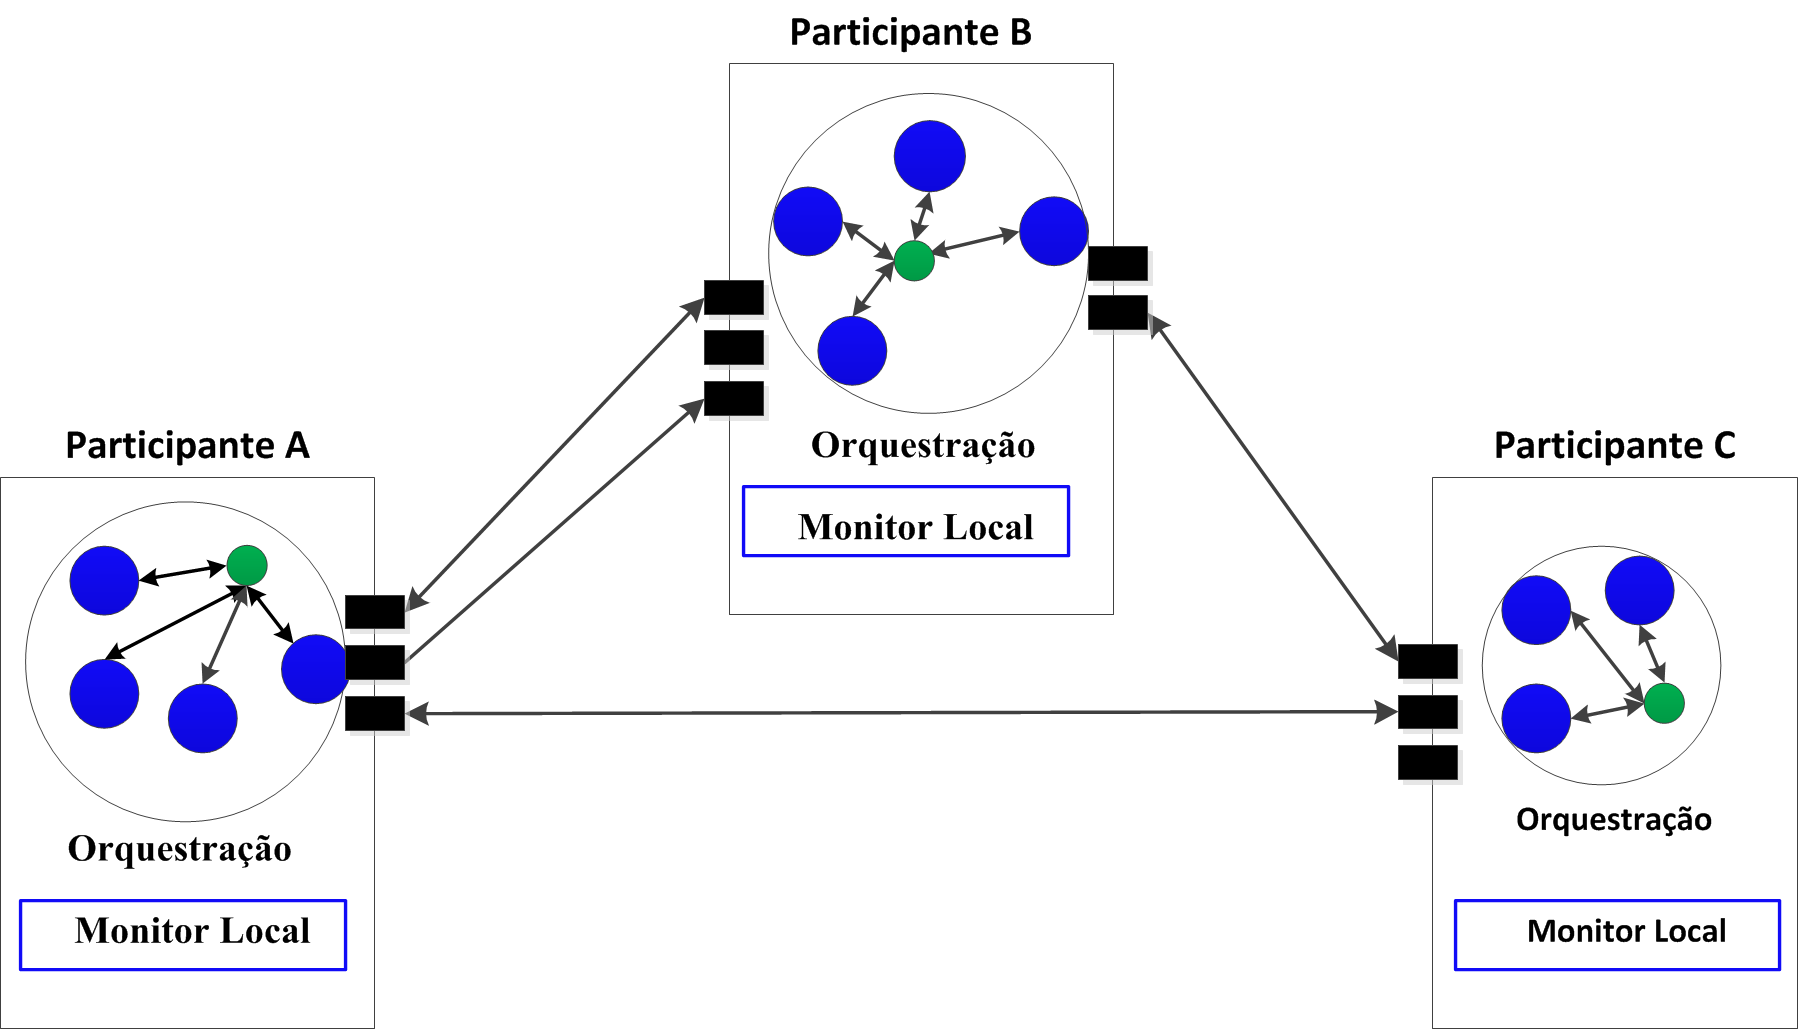
\includegraphics[width=0.9\textwidth]{MonitoringOverview_2.png}
              \caption{Perspectiva Geral do monitoramento proposto}
          \end{figure}	
      }
       \only<3>{	
          \begin{figure}
              \centering
              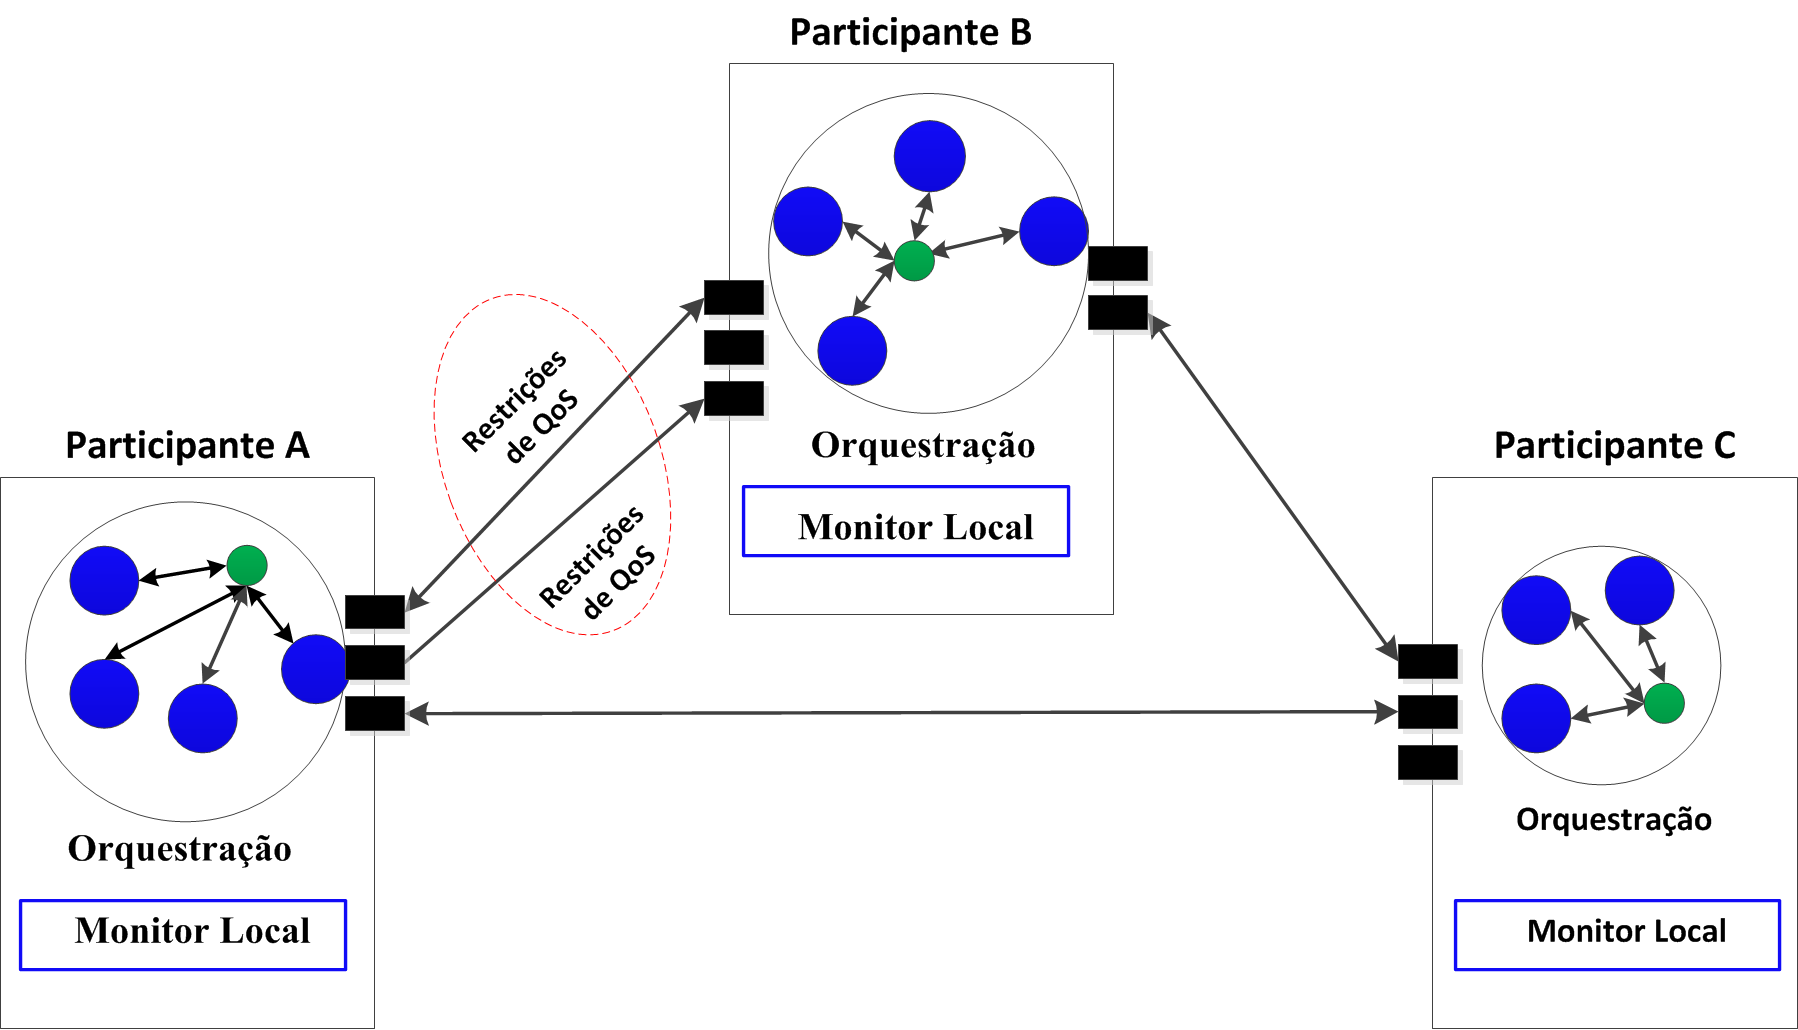
\includegraphics[width=0.9\textwidth]{MonitoringOverview_3.png}
              \caption{Perspectiva Geral do monitoramento proposto}
          \end{figure}	
      }

       \only<4>{	
          \begin{figure}
              \centering
              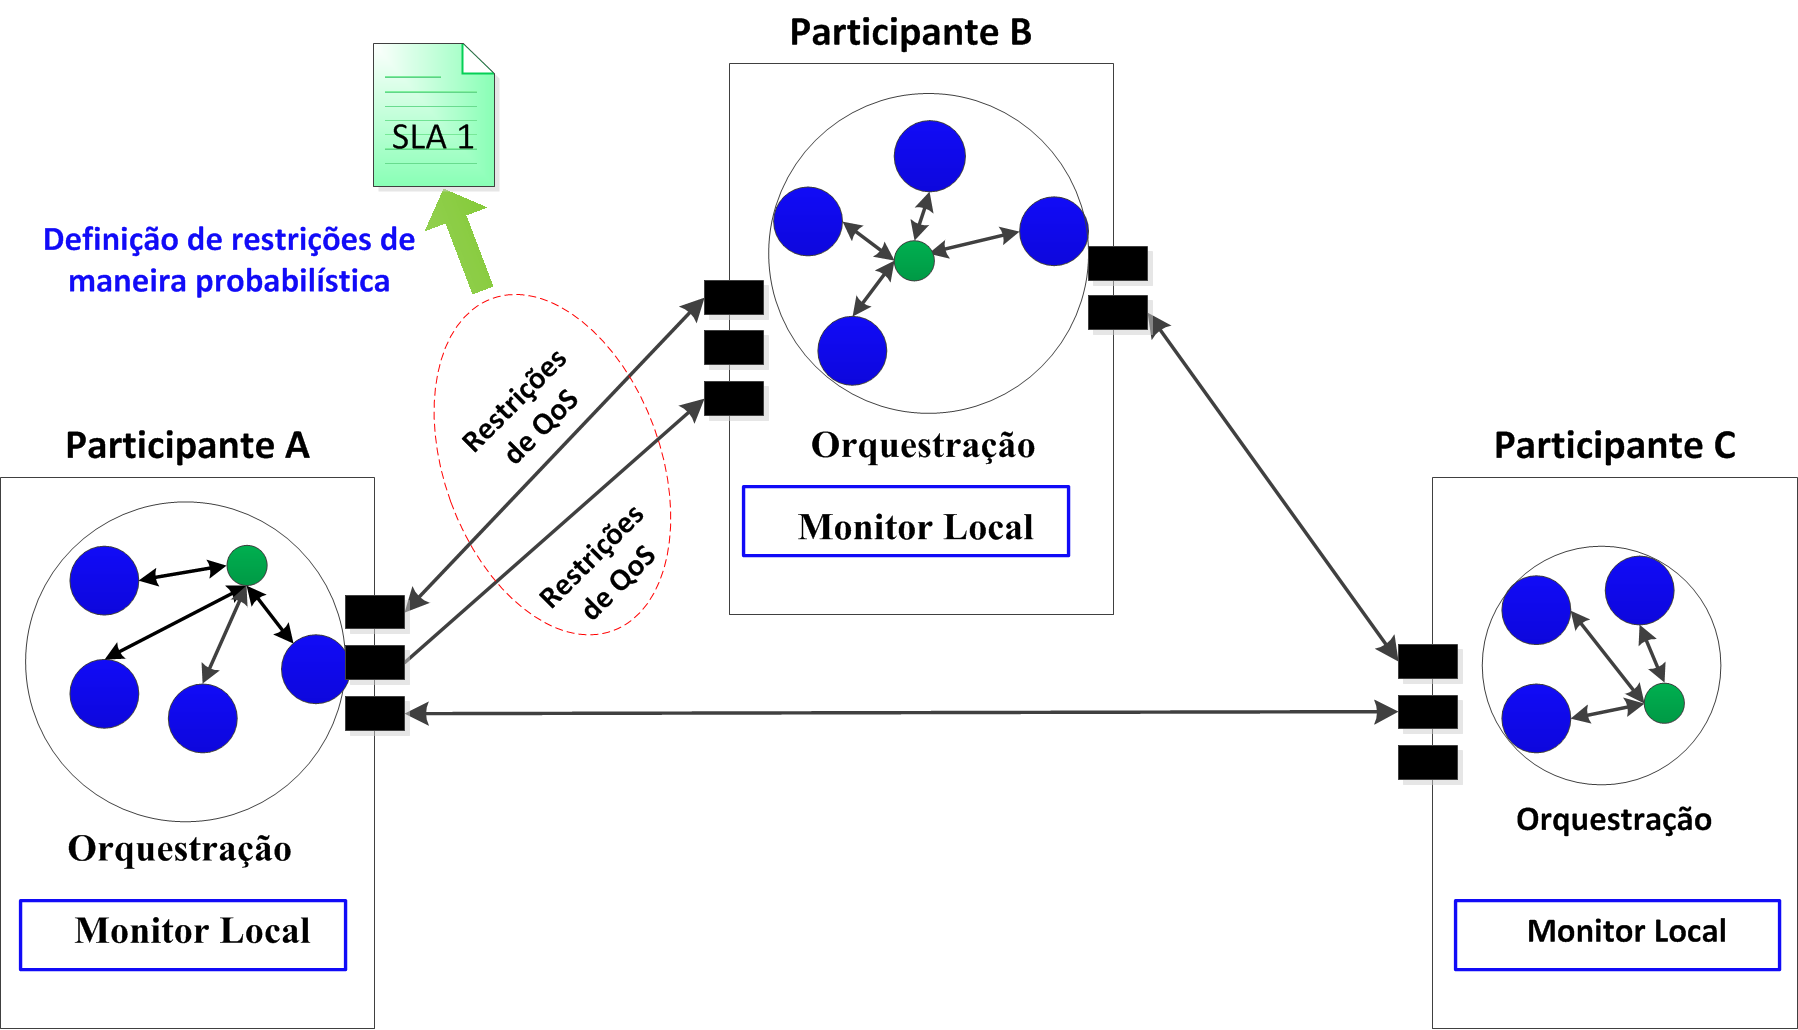
\includegraphics[width=0.9\textwidth]{MonitoringOverview_4.png}
              \caption{Perspectiva Geral do monitoramento proposto}
          \end{figure}	
      }

       \only<5>{	
          \begin{figure}
              \centering
              \includegraphics[width=0.9\textwidth]{MonitoringOverview_5.png}
              \caption{Perspectiva Geral do monitoramento proposto}
          \end{figure}	
      }

       \only<6>{	
          \begin{figure}
              \centering
              \includegraphics[width=0.80\textwidth]{MonitoringOverview_6.png}
              \caption{Perspectiva geral do monitoramento proposto}
          \end{figure}	
      }

      \only<7>{	
          \begin{figure}
              \centering
              \includegraphics[width=0.8\textwidth]{MonitoringOverview_7.png}
              \caption{Perspectiva geral do monitoramento proposto}
          \end{figure}	
      }
    \end{frame}

  \begin{frame}{ Modelo de QoS  (I)}
    \begin{itemize} %%Perhaps it's needed use some picture, for example life cycle call service.
	%\item Os atributos de QoS envolvem: \textbf{service}, \textbf{network} and \textbf{message} aspects.
	\item Atributos de QoS:
	    \begin{itemize}
	      \item <2->\colorbox{yellow}{Serviço}: \textbf{tempo de processamento, tempo de resposta, }.
	      \item <3->\colorbox{yellow}{Rede}: largura de banda, atraso e \textbf{erros de comunicação}.
	      \item <4->\colorbox{yellow}{Mensagem}: \textbf{integridade da mensagem}.
	    \end{itemize}
    \end{itemize}
  \end{frame}

  \begin{frame}{ Modelo de QoS  (II)}
    \only<1>{	
	\begin{figure}[h]
	    \centering
	    \includegraphics[width=.6\linewidth]{figures/ChorInteractionToServiceInteraction.png}
	    \caption{ Interação de serviços a partir de  interações atômicas do BPMN2.}
	    \label{figure:InteractionBPMNServiceInteraction}
	\end{figure}
    }
    \only<2>{	
	\begin{figure}[h]
	    \centering
	    \includegraphics[width=.6\linewidth]{figures/QoSInvocationService.png}
	    \caption{Atributos de QoS em uma interação com um serviço Web.}
	    \label{figure:QoSInvocationService}
	\end{figure}
    }
  \end{frame}


%%Formulas?


\subsection{Definição de requisitos de QoS}
  \begin{frame}{Definição de requisitos de QoS: Analiticamente}
      \begin{enumerate}
	\item <1-> \textbf{Mapeamento} de uma coreografia para uma GSPN ( Rede Petri Estocástica Generalizada).
	    %\begin{itemize}
	    %  \item The choreography is specified according to ``interaction model''.
	    %  \item The choreography is specified in BPMN 2.0.
	    %  \item The resulting GSPN include a QoS model.
	    %\end{itemize}

	\item <2-> \textbf{Configurações} na GSPN obtida.
	\item <3-> \textbf{Simulações} dos cenários.
      \end{enumerate}

  \end{frame}
  

  \begin{frame}{Mapeamento de BPMN para GSPN (I)}
      \only<1>{
	  \begin{figure}[!h]
	  \centering
	  \includegraphics[width=0.8\textwidth]{BPMNChoreographyElements2_a.png}
	  \caption{Mapeamento de eventos e \textit{gateways} para módulos GSPN.}
	\end{figure}
      }
      \only<2>{
	\begin{figure}[!h]
	  \centering
	  \includegraphics[width=0.8\textwidth]{BPMNChoreographyElements2_b.png}
	  \caption{Mapeamento de eventos e \textit{gateways} para módulos GSPN.}
	\end{figure}
      }
    
  \end{frame}


  \begin{frame}{Mapeamento de BPMN para GSPN (II)}
	\only<1>{	
	      \begin{figure}[!h]
		  \centering
		  \includegraphics[width=1.0\textwidth]{BPMNTaskChoreography-QoS_Model_a-br.png}
	      \end{figure}
	  }
	  \only<2>{	
	      \begin{figure}[!h]
		  \centering
		  \includegraphics[width=1.0\textwidth]{BPMNTaskChoreography-QoS_Model_b-br.png}
	      \end{figure}
	  }

	\only<3>{	
	      \begin{figure}[!h]
		  \centering
		  \includegraphics[width=1.0\textwidth]{BPMNTaskChoreography-QoS_Model_1-br.png}
	      \end{figure}
	  }
	\only<4>{	
	      \begin{figure}[!h]
		  \centering
		  \includegraphics[width=1.0\textwidth]{BPMNTaskChoreography-QoS_Model_2-br.png}
	      \end{figure}
	  }
      \only<5>{
	      \begin{figure}[!h]
		  \centering
		  \includegraphics[width=1.0\textwidth]{BPMNTaskChoreography-QoS_Model_3-br.png}
	      \end{figure}
      }
      \only<6>{
	      \begin{figure}[!h]
		  \centering
		  \includegraphics[width=1.0\textwidth]{BPMNTaskChoreography-QoS_Model_4-br.png}
	      \end{figure}
      }
      \only<7>{
	      \begin{figure}[!h]
		  \centering
		  \includegraphics[width=1.0\textwidth]{BPMNTaskChoreography-QoS_Model_5-br.png}
	      \end{figure}
      }
  \end{frame}


  \begin{frame}{Algoritmo de Mapeamento (I)}
      \begin{algorithm}[H]
	  %\caption{Mapping a Interconnection Choreography in BPMN onto a GSPN with QoS model}
	    %\caption{ { \small Mapeamento de uma coreografia especificada em BPMN 2.0 para uma GSPN com o modelo de QoS } }
	    \caption*{ Mapeamento de uma coreografia em BPMN 2.0 para uma GSPN com suporte de QoS}
	    %\label{alg2}

	    \begin{algorithmic}%[1]
	      { \footnotesize		
			    %\REQUIRE Process Choreography $\mathcal{PC}$ in BPMN 2.0.
			    \visible<1->{ \REQUIRE \textbf{Process Choreography} \textcolor{componentColor}{ \textbf{ $PC = (\mathcal{O, A, E, G, T}, \{e^S\}, \mathcal{E}^I,$ $\{e^E\}, \mathcal{E}^{I_M}, \mathcal{E}^{I_T},
			    \mathcal{G}^F, \mathcal{G}^J,$ $\mathcal{G}^X, \mathcal{G}^M, \mathcal{G}^V, \mathcal{F} )$} } in BPMN 2.0. }

			    \visible<2->{ \ENSURE Generalized Stochastic Petri Net \textcolor{componentColor}{ \textbf{$GSPN_{QoS}$} }.  }
			    \vspace*{3 mm}	
	      }	
		{ \tiny	
			  \visible<3->{
		      \STATE \textcolor{componentColor}{ \textbf{$CT_i \in \mathcal{T} $, $G_j \in \mathcal{G} $}} and \textcolor{componentColor}{ \textbf{$E_k \in \mathcal{E}$}. where  $i, j, k \in \mathbb{N} $}.
			    %\STATE Let $PNQoS(CT_i)$ a respective GSPN including QoS from type of $CT_i$ and according to mapping rules (Figure \ref{fig:MappingTaskChoreographiesQoS1}).
			    %\STATE Let $PNQoS(CT_i)$ be a respective GSPN including QoS from type $CT_i$ and according to mapping rules (Figure \ref{fig:MappingTaskChoreographiesQoS1}).
		      
	      %	      \visible<4->{ \STATE \textcolor{componentColor}{ $PNQoS(CT_i)$, $PNQoS(G_j)$, $PNQoS(E_k)$   } are functions of the type %of \textcolor{componentColor}{ $CT_i$, $G_j$, $E_k$} respectively that return a GSPN according to mapping rules. }

			    \STATE \textcolor{componentColor}{ $PNQoS(CT_i)$, $PNQoS(G_j)$, $PNQoS(E_k)$   } are functions return a GSPN according to mapping rules.

			    \STATE \textcolor{componentColor}{ {\normalsize \textbf{$\oplus$}} } as the operator composition that returns other GSPN. 
			    \vspace*{3 mm}
			    \STATE $\textcolor{componentColor}{GSPN_{QoS} } \leftarrow  Empty\  Petri\  Net$

			    %\FOR { $CT_i \in T $ }
			    % \STATE $GSPN_{QoS} \leftarrow GSPN_{QoS} \oplus PNQoS(CT_i)$
			    %\ENDFOR

			  \FOR { $\textcolor{componentColor}{ CT_i} \in \textcolor{componentColor}{\mathcal{T}} $ }
			      \STATE $\textcolor{componentColor}{ GSPN_{QoS} } \leftarrow \textcolor{componentColor}{ GSPN_{QoS} } \oplus \textcolor{componentColor}{ PNQoS(CT_i) } $  		
			      \STATE Add a arrival \textbf{timed Transition} at beginning of the \textcolor{componentColor}{$GSPN_{QoS}$}.
			  \ENDFOR
			    %\vspace*{3 mm}
			  \FOR{ $\textcolor{componentColor}{G_j} \in \textcolor{componentColor}{\mathcal{G}} $ } 			
			      \STATE $\textcolor{componentColor}{ GSPN_{QoS} } \leftarrow \textcolor{componentColor}{GSPN_{QoS}} \oplus \textcolor{componentColor}{ PN(G_j) }$	
			  \ENDFOR	
			  %\vspace*{3 mm}
			  \FOR{ $\textcolor{componentColor}{ E_k } \in \textcolor{componentColor}{ \mathcal{E} } $ }					 	
			      \STATE $\textcolor{componentColor}{ GSPN_{QoS} } \leftarrow \textcolor{componentColor}{ GSPN_{QoS} } \oplus \textcolor{componentColor}{ PN(E_k) }$  	
			  \ENDFOR

			  \STATE Add a starting Place and \textbf{immediate Transition} at the beginning of the \textcolor{componentColor}{ $GSPN_{QoS}$}.	
			  \STATE Add a ending Place and \textbf{immediate Transition} at the end of the \textcolor{componentColor}{$GSPN_{QoS}$}.	

			  \RETURN \textcolor{componentColor}{$GSPN_{QoS}$}
		}
	      }	
	
	\end{algorithmic}

      \end{algorithm}
  \end{frame}


 \begin{frame}{ Algoritmo de Mapeamento (II)}
    \only<1>{	
        \begin{figure}[!h]
            \centering
            \includegraphics[width=0.5\textwidth]{Algorithm1.png}
        \end{figure}
    }
    \only<2>{	
        \begin{figure}[!h]
            \centering
            \includegraphics[width=0.5\textwidth]{Algorithm2.png}
        \end{figure}
    }
    \only<3>{	
        \begin{figure}[!h]
            \centering
            \includegraphics[width=0.65\textwidth]{Algorithm3.png}
        \end{figure}
    }
    \only<4>{	
        \begin{figure}[!h]
            \centering
            \includegraphics[width=0.65\textwidth]{Algorithm4.png}
        \end{figure}
    }
 \end{frame}




%\subsection{ChorSim: Simulador de Coreografias}
  \begin{frame}{ChorSim: Simulador de Coreografias}
  
     \only<1>{
	\begin{figure}[!h]
	  \centering
	  \includegraphics[width=.6\linewidth]{figures/ServiceDependency_Events_QoS.png}
	  \caption{Atributos de QoS calculados em um evento dado. (1) Recebendo requisições de um cliente ou serviço. (2) enviando
	  requisições para um outro serviço. (3) recebendo resposta de um outro serviço (dependência). (4) enviando resposta para um cliente ou serviço solicitador.}
	  \label{figure:QoSAttributosEvents}
	\end{figure}
    }
    \only<2>{
      \begin{figure}
	  \centering
	  \includegraphics[width=0.7\textwidth]{figures/Architecture-Simulator.png}
	  % MonitoringOverview.png: 1756x1462 pixel, 250dpi, 17.84x14.85 cm, bb=0 0 506 421
	  \caption{Arquitetura do simulador de coreografias.}
	  \label{fig:chorsim_architecture}
	\end{figure}
    }
  
  \end{frame}


%%TODO:  Mais imagens pro simulador, troços de código?



  \subsection{Estabelecimento do contrato probabilístico}

  \begin{frame}{Estabelecimento de SLAs Probabilísticos}

        \textcolor{Blue}{$$F_S(x) = P(\delta_S \leq x)$$ } é a função distribuição acumulada (fda) de um parâmetro
       de QoS \textcolor{Blue}{$\delta$} do serviço \textcolor{Blue}{$S$}.
      \pause

      \begin{enumerate}
      \item <1->\textbf{Condições Iniciais}:
	  \begin{itemize}
	    \item <1-> Configurar a plataforma e a implantação no ChorSim.
	    \item <2-> Estimar a função de distribuição acumulada \textcolor{Blue}{$Fs_i$} para cada  serviço \textcolor{Blue}{$S_i$}.
	    %\item <3-> Definir os quantis que representem todo \textcolor{Blue}{$Fs_i$}.
	  \end{itemize}

      \item <3-> \textbf{Simulação usando \textbf{ChorSim}}:
	  \begin{enumerate}
	  \item <3-> \label{a} Para cada invocação de um serviço \textcolor{Blue}{$s_i$} na interação de um participante
	    provedor A com um outro participante cliente B, um valor do parâmetro de QoS \textcolor{Blue}{$q$}
	    é obtido a partir da simulação em ChorSim.%de \textcolor{Blue}{$Fs_i(x)$}.
	  \item <4-> \label{b} \textbf{Agregação}: Estimar o valor do parâmetro de QoS do serviço composto $S$ a partir dos valores obtidos
	  no passo anterior usando o ChorSim. %precisa de um modelo (ex.: modelo de execução de ordens parciais)

	  \item <5-> Rodar as simulações dos passos 2.1 e 2.2 várias vezes, o suficiente para estimar  empiricamente \textcolor{Blue}{$F_S$}.%end-to-end
	  \end{enumerate}

	\item <6-> A partir de \textcolor{Blue}{$F_S$}  se selecionam quantis para definir o contrato.

     % simulação com o método de Monte-Carlo:
    \end{enumerate}
  \end{frame}

  

\subsection{Monitoramento de coreografias }


  % ---- Monitoramento Probabilístico de Coreografias%
  \begin{frame} { Monitoramento }

      \begin{itemize}
	\item \textcolor{Blue}{$F_S$}:  Distribuição de probabilidade do contrato.
	\item \textcolor{Blue}{$\Delta$}: Um conjunto finito de amostras dos valores de um parâmetro de QoS do serviço \textcolor{Blue}{$S$}.
	%\item \textcolor{Blue}{$f'_{si}$}: Distribuição de probabilidade empírica de um serviço.
	%\item Agregação de QoS.
	\item \textcolor{Blue}{$F'_S$}: Distribuição de Probabilidade após a agregação usando ChorSim.
	%\item \textcolor{Blue}{$F_s$} : Função Distribuição de Probabilidade parâmetro de QoS \textcolor{Blue}{$p$} do %serviço composto \textcolor{Blue}{$S$}.
	\item \textcolor{Blue}{$\lambda$}: Zona de Tolerância.
      \end{itemize}


        \begin{equation}
            \textcolor{Blue}{
                F'_{S,\Delta}(x) = \frac{ | \{\delta, \delta \in \Delta \leq x  \}|}{|\Delta|}
            }
        \end{equation}
    	
	\pause
        %\begin{equation}
        %\textcolor{Blue}{
        %    \forall x \in R^{+} : F'_{s,\Delta}(x) \geq F_s(x)
        %     }
        %\end{equation}

        \begin{equation}
            \textcolor{Blue}{
                 \exists x \in R^{+} : F'_{s,\Delta}(x) < F_s(x)
            }
        \end{equation}

	\pause
	%\colorbox{yellow}{\parbox{0.5\textwidth}{
        \begin{equation}
            \textcolor{Blue}{
              sup_{x \in R^+}  (F'_{s,\Delta}(x) - F_s(x) ) \geq \lambda  \footnote{Rosario et al., 2009}
            }
        \end{equation}
	%}}
  \end{frame}


  \begin{frame}{ Detecção de Violações de SLA (I)}
      \textbf{Problema:} Dominância estocástica

      \begin{equation}	\textcolor{Blue}{
	\begin{align}
	  H_0 : & \quad \forall x, F_S(x) >=F'_S(x)   \notag\\
	  contra \notag\\
	  H_1 : &  \quad \exists x, F_S(x) < F'_S(x) 
	\end{align}}
      \end{equation}
      \pause 
    \textbf{Solução:} \textit{One-sided two-sample Kolmogorov-Smirnov test} 

      \begin{equation}	\textcolor{Blue}{
	  [D,p] = kstest(X_{contract}, X_{monitoring}, KS_{side})
	}
      \end{equation}
  \end{frame}

%%TODO: precisa-se explica ro que é KS com graficos e tudo o mais?

  \begin{frame}{Detecção de Violações de SLA (II)}
    Então, para a detecção de violações usam-se:
      \begin{equation*} 	\textcolor{Blue}{
	\begin{align}
	  [D^{+},p^{+}] & = kstest(X_{contract}, X_{monitoring}, greater) \notag\\
	  [D^{-},p^{-}] & = kstest(X_{contract}, X_{monitoring}, less)
	\end{align} }
      \end{equation*} 

    \pause
    Portanto,  para que um conjunto de amostras \textcolor{Blue}{$X_{monitoring}$} cumpra o contrato uma regra baseada
    em \textcolor{Blue}{$p^{+}$} e \textcolor{Blue}{$D$} deve ser definida:

    \pause
      \begin{equation*}
	\textcolor{Blue}{
	  verify(X_{monitoring}) = 	
	  \begin{cases}
	  true,  & \text{ se } p^{+}>= \alpha \wedge D^{+}< \lambda \\
	  false, &  \text{ de outra maneira }
	  \end{cases}
	}
      \end{equation*}
    

  \end{frame}




% ------------------------------------------------------------------%
% -------------    Experimentos e Resultados   ---------------------%
% ------------------------------------------------------------------%
\section{Experimentos e Resultados}
\subsection{ Definição de Requisitos de QoS Analiticamente}

  \begin{frame}{Cenário de Coreografia para a abordagem analítica}
    \begin{figure}[!h]
	\centering
	\includegraphics[width=0.7\textwidth]{figures/Example-InteractionChor-br.png}
	\caption{Exemplo de modelo de interação de coreografias, oferta de investimento. }%Interconnection model describing investment offers 
	\label{fig:Example-InteractionChor}
    \end{figure}
  \end{frame}

  \begin{frame}{Mapeamento}
    \begin{figure}[!h]
    	\centering
    	\includegraphics[width=1.0\textwidth]{BPMNChoreographyExample-QoS.png}
    	\caption{GSPN obtida após o mapeamento.}
    \end{figure}
  \end{frame}



  \begin{frame}{ Configuração (I)}
      \only<1>{
	      \begin{figure}[!h]
		  \centering
		  \includegraphics[width=1.0\textwidth]{BPMNChoreographyExample-QoS_configuration1-br.png}
	      \end{figure}
      }
      \only<2>{
	      \begin{figure}[!h]
		  \centering
		  \includegraphics[width=1.0\textwidth]{BPMNChoreographyExample-QoS_configuration2-br.png}
	      \end{figure}
      }
      \only<3>{
	      \begin{figure}[!h]
		  \centering
		  \includegraphics[width=1.0\textwidth]{BPMNChoreographyExample-QoS_configuration3-br.png}
	      \end{figure}
      }
      \only<4>{
	      \begin{figure}[!h]
		  \centering
		  \includegraphics[width=1.0\textwidth]{BPMNChoreographyExample-QoS_configuration4-br.png}
	      \end{figure}
      }
      \only<5>{
	      \begin{figure}[!h]
		  \centering
		  \includegraphics[width=1.0\textwidth]{BPMNChoreographyExample-QoS_configuration5-br.png}
	      \end{figure}
      }
      \only<6>{
	      \begin{figure}[!h]
		  \centering
		  \includegraphics[width=1.0\textwidth]{BPMNChoreographyExample-QoS_configuration6-br.png}
	      \end{figure}
      }
      \only<7>{
	      \begin{figure}[!h]
		  \centering
		  \includegraphics[width=1.0\textwidth]{BPMNChoreographyExample-QoS_configuration7-br.png}
	      \end{figure}
      }
  \end{frame}

  \begin{frame}{ Configuração (II) }
        \begin{table}[!h]
            \centering
            \caption{Pesos dos cenários 1 e 2}
            \label{table:transitionsConfigurations}
            \begin{tabular}{ lcc}
              %\cline{1-3}
	      \toprule	
        		    &   \multicolumn{2}{c}{ \textbf{Pesos} } \\
              %\cline{1-3}
	      \cmidrule(r){2-3}
              %\hline
              \textbf{Transição}      		&      \textbf{Cenário 1}   &  \textbf{ Cenário 2} 		\\
               %\hline
	      \otoprule
               $T_{latency1}$, $T_{latency2}$, $T_{latency3}$ 	& 	0.99       &   0.94	\\
               $T_{cerr1}$, $T_{cerr2}$, $T_{cerr3}$      	&  	0.01 	   &   0.06	\\
               $T_{receive}$, $T_{receive2}$, $T_{receive3}$  &  	99  	   &    97	\\
               $T_{merr1}$, $T_{merr2}$, $T_{merr3}$   &   1 	   &    3	\\
               $T_{arrival2}$, $T_{arrival3}$   &  0.5  &	0.5	\\
              \bottomrule
            \end{tabular}
        \end{table}

  \end{frame}


    \begin{frame}{ Simulações na GSPN }
      \begin{itemize}
	\item <1-> A ferramenta \textbf{Pipe2} foi usado para \textbf{modelar} e \textbf{simular} a \textbf{GSPN}.
	\item <2-> \textbf{$1$ token} = \textbf{$1$ instância de coreografia}.
	\item <2-> \textbf{$100$ tokens} são considerados para cada cenários na posição de inicio (\textbf{Start}).
	\item <2-> \textbf{$100$ instâncias concorrentes} foram executadas (\textit{multiple-server semantic}).
	\item <3-> $1500$ disparos e $10$ replicações.
	\item <3-> Nível de confiança de $95\%$.
      \end{itemize}
    \end{frame}

    \begin{frame}{ Resultados }
	\only<1>{
	  \begin{table} [tp] %[!h]
		\centering
		\caption{Resultados das simulações} % (in \%) }
		\begin{figure}[!h]
		    \centering
		    \includegraphics[width=0.9\textwidth]{results1-gspn.png}
		\end{figure}
	  \end{table}
	}
	\only<2>{
	  \begin{table} [tp] %[!h]
		\centering
		\caption{Resultados das simulações} % (in \%) }
		\begin{figure}[!h]
		    \centering
		    \includegraphics[width=0.9\textwidth]{results2-gspn.png}
		\end{figure}
	  \end{table}
	}
	\only<3>{
	  \begin{table} [tp] %[!h]
		\centering
		\caption{Resultados das simulações} % (in \%) }
		\begin{figure}[!h]
		    \centering
		    \includegraphics[width=0.9\textwidth]{results3-gspn.png}
		\end{figure}
	  \end{table}
	}
	\only<4>{
	  \begin{table} [tp] %[!h]
		\centering
		\caption{Resultados das simulações} % (in \%) }
		\begin{figure}[!h]
		    \centering
		    \includegraphics[width=0.9\textwidth]{results4-gspn.png}
		\end{figure}
	  \end{table}
	}
  \end{frame}


\subsection{Definição de requisitos de QoS usando ChorSim}
%% Definição de requisitos de QoS usando ChorSim
  \begin{frame}{Cénario de coreografia para a abordagem com ChorSim}
    \begin{figure}[h]
	\centering
	%\subfloat[orchestrated version\label{fig:commDiaOrch}]{\includegraphics[width=.5\linewidth]{figures/orchestration}}
	%\subfloat[choreographed version\label{fig:commDiaChor}]{\includegraphics[width=.5\linewidth]{figures/choreography}}
	\includegraphics[width=.8\linewidth]{figures/CDN_choreography-scenario.png}
	\caption{Coreografia de serviços da aplicação de CDN}
	\label{figure:scenario}
    \end{figure}
  \end{frame}


  \begin{frame}{Configuração das simulações em ChorSim (I)}  
      
      \begin{block}{Objetivo} 
      Analisar o comportamento do \textbf{tempo de resposta total} do serviço composto $WS_1$ em função do
      \textbf{tamanho da resposta} de $WS_1$ e diferentes valores de \textbf{largura de banda}.
      \end{block}

      \pause 

    \only<2>{
      \begin{itemize}
	\item \textbf{Cenário 1:}   Larguras de banda uniformes.
	\item \textbf{Cenário 2:}   Larguras de banda váriaveis.
      \end{itemize}
     }
    
  \end{frame}

  \begin{frame}{Configuração das simulações em ChorSim (II)}  
	\textbf{Cenario 2:}
  	\begin{figure}[!h]
	    \centering
	    %\subfloat[orchestrated version\label{fig:commDiaOrch}]{\includegraphics[width=.5\linewidth]{figures/orchestration}}
	    %\subfloat[choreographed version\label{fig:commDiaChor}]{\includegraphics[width=.5\linewidth]{figures/choreography}}
	    \includegraphics[width=1.0\linewidth]{figures/failure_model.png}
	    \caption{Cenário 2:Largura de banda efetiva devido à degradação da largura de banda referencial em um período de $100$ segundos.}
    %       \caption{Capacidade variável da Largura de Banda  referencial em um período de tempo de $100$ segundos}
	    \label{figure:failure_model}
	\end{figure}
  \end{frame}  

  \begin{frame}{Configuração das simulações em ChorSim (III)}  
      \begin{table}[!h]
	    \centering
      {\footnotesize
	    \caption{Configuração de valores dos atributos de QoS nas requisições}
	    \label{table:simulation_configuration_responses}
	  \begin{tabular}{|l|c|c|c|c|}
		%%\hline
			    %%& \multicolumn{2}{c|}{ Average number of tokens } & \multicolumn{2}{c|}{ 95\% Confidence interval  (+/-) }\\
		\hline
		\textbf{Requisições}           &  Largura de banda     &   Tamanho da requisição    &  Latência       &  \# requisições	  \\
		\hline
		$Cliente$ a $WS_1$    &    $1$Mbps	              &      $1.95$MB        &   $0.002s$      &     $1$ a $10$     \\
		$WS_1$ a $WS_3$       &    $1$Mbps	              &      $5.47$MB        &   $0.002s$      &     $1$ a $10$     \\
		$WS_3$ a $WS_5$       &    $1$Mbps                  &      $5.47$MB        &   $0.002s$      &       $1$ a $10$     \\
		\hline
		\end{tabular}
      }
      \end{table}

      \pause
      \begin{table}[!h]
	    \centering
      {\footnotesize
	    \caption{Configuração de valores dos atributos de QoS nas respostas}
	    \label{table:simulation_configuration_requests}
	  \begin{tabular}{|l|c|c|c|c|}
		%%\hline
			    %%& \multicolumn{2}{c|}{ Average number of tokens } & \multicolumn{2}{c|}{ 95\% Confidence interval  (+/-) }\\
		\hline
		\textbf{Respostas}           &  Largura de banda           &   Tamanho de resposta    &  Latência         &   \emph{timeout}	  \\
		\hline
		$WS_1$ a $Cliente$  &    $1$Mbps a $16$Mbps	        &    $1$KB a  $100$MB                   &   $0.002s$      &   $1000s$     \\
		$WS_3$ a $WS_1$     &    $20$Mbps	                &      $8$MB                   &   $0.002s$      &   $1000s$     \\
		$WS_5$ a $WS_3$     &    $40$Mbps                 &      $200$MB                 &   $0.002s$      &   $1000s$     \\
		\hline
		\end{tabular}
      }
      \end{table}
  \end{frame}

  
  \begin{frame}{Resultados das simulações usando ChorSim}
    \only<1>{
      \framesubtitle{Cenário 1}    
      \begin{figure}[H]
	  \centering
	  %\subfloat[orchestrated version\label{fig:commDiaOrch}]{\includegraphics[width=.5\linewidth]{figures/orchestration}}
	  %\subfloat[choreographed version\label{fig:commDiaChor}]{\includegraphics[width=.5\linewidth]{figures/choreography}}
	  \includegraphics[width=1.0\linewidth]{figures/results1-normal.png}
	  \caption{\textbf{Cenario 1:} Tempo médio de resposta total da coreografia em função do tamanho de resposta do serviço $WS_1$ com
	  larguras de banda de $1Mbps$ até	$16Mbps$}
	  \label{figure:results}
      \end{figure}
    }
    \only<2>{
      \framesubtitle{Cenário 2}    
      \begin{figure}[H]
	  \centering
	  %\subfloat[orchestrated version\label{fig:commDiaOrch}]{\includegraphics[width=.5\linewidth]{figures/orchestration}}
	  %\subfloat[choreographed version\label{fig:commDiaChor}]{\includegraphics[width=.5\linewidth]{figures/choreography}}
	  \includegraphics[width=1.0\linewidth]{figures/results1-failure.png}
	  \caption{\textbf{Cenário 2:} Tempo médio de resposta total da coreografia em função do tamanho de resposta do serviço $WS_1$.
		    A largura de banda varia de $1Mbps$ até $16Mbps$}
	  \label{figure:results_failure}
      \end{figure}
    }
  \end{frame}  


%%%
\subsection{Estabelecimento do contrato de QoS}

  \begin{frame}{Estabelecimento do contrato probabilístico (I)}
      \begin{table}[!h]
	    \centering
      {\footnotesize
	    \caption{Configuração das taxas de degradação dos serviços  para obter o contrato do tempo de resposta para o serviço composto $WS_1$ }
	    \label{table:contract_configurations}
	  \begin{tabular}{ccc}
		%%\hline
			    %%& \multicolumn{2}{c|}{ Average number of tokens } & \multicolumn{2}{c|}{ 95\% Confidence interval  (+/-) }\\
		\toprule
		\textbf{Serviço}    &   \textbf{Distribuição}      &     \textbf{Taxa de degradação ($\lambda$)}      \\
		\otoprule
		$WS_1$     &    Exponencial      &      1/10000      \\
		$WS_3$     &    Exponencial      &      1/10000      \\
		$WS_5$     &    Exponencial      &      1/10000      \\
		\bottomrule
		\end{tabular}
      }
      \end{table}
  \end{frame}
  

  \begin{frame}{Estabelecimento do contrato probabilístico (II)}
    \begin{figure}[H]
	\centering
	\includegraphics[width=1.0\linewidth]{figures/contract.png}
	\caption{Distribuição de probabilidade empírica (ECDF) do contrato do serviço $WS_1$ com base nos tempos de resposta  }
	\label{figure:contract}
    \end{figure}
  \end{frame}


%%%
\subsection{Monitoramento}

  \begin{frame}{Configuração do Monitoramento}
    \begin{equation}
      \textcolor{Blue}{
	  verify(X_{monitoring}) = 	
	  \begin{cases}
	  true,  &  \text{ se } p^{+}>= 0.05 \wedge D^{+} < 0.15 \\
	  false, &  \text{ de outra maneira }
	  \end{cases}
      }
    \end{equation}
  
    \pause
    \begin{itemize}
      \item \textcolor{Blue}{$X_{monitoring}$}: Conjunto de amostras dos tempos de resposta do serviço composto \textcolor{Blue}{$WS_1$}. 
      \item Um monitoramento sequencial e  \textit{on-line} precisa  computar  $N$ amostras que que se sobrepõem. 
      \item Conjunto de janelas de  amostras a monitorar: 
	    \begin{itemize}
	     \item [] \textcolor{Blue}{$\{1, \dots , N\}, \{p, \dots , p + N\}, \dots , \{mp, \dots ,mp + N\} \dots$ }
	     \item [] \textcolor{Blue}{$p <=N $} e \textcolor{Blue}{$m=1, 2,\dots \quad$ }
	    \end{itemize}

      \item Configuração: \textcolor{Blue}{$N = 100$}, e o desvio \textcolor{Blue}{$p=1$}.
    \end{itemize}

  \end{frame}


%\colorbox{green!25}{}
%\colorbox{red!25}{$3.10\%$}
  \begin{frame}{Cenários para o monitoramento}
    \begin{center}
      \begin{table}[h]
	  \centering
	\caption{ Estabelecimento das taxas de degradação de tempo de processamento dos serviços para os cenários.  }
	\begin{center}
	  \begin{tabular}{ cccc}
	    %\hline
	    % after \\: \hline or \cline{col1-col2} \cline{col3-col4} ...
	    \toprule
			&   \multicolumn{3}{c}{ \textbf{Taxa de degradação ($\lambda$)} } \\
	    %\cline{1-4}
	    %\cmidrule{1-4}
	    \textbf{Cenário}    &    $WS_1$	  &	  $WS_3$ 	& 	 $WS_5$ \\
	    %\otoprule
	    \cmidrule[1pt](r){1-1} \cmidrule[1pt](l){2-4}
	    %\rowcolor{yellow!35}
	    
	    %25\% & 2.5 ms \\
	    %50\% & 4.5 ms \\
	    %\rowcolor{red!25}
	    %\midrule
	    Cenário 1 &		\cellcolor{red!25} 1/13000  	 & 	\cellcolor{red!25} 1/12500		&	\cellcolor{red!25} 1/11500	\\
	    %\rowcolor{red!25}
	    Cenário 2 &		\cellcolor{red!25} 1/12000  	 & 	\cellcolor{red!25} 1/11000		&	\cellcolor{red!25} 1/12000	\\
	    %Cenário 3 &	1/11000  	 & 	1/10500		&	1/11000	\\
	    %Cenário 4 &	1/10000  	 & 	1/11000		&	1/10000	\\
	    \midrule
	    %\rowcolor{green!25}
	    Cenário 3 &		\cellcolor{green!25} 1/10500  	 & 	\cellcolor{green!25} 1/10000		&	\cellcolor{green!25} 1/10500	\\
	    %\rowcolor{green!25}
	    Cenário 4 &		\cellcolor{green!25} 1/9000  	 & 	\cellcolor{green!25} 1/10000		&	\cellcolor{green!25} 1/9000	\\
	    %\hline
	    %\midrule
	    \cmidrule[1pt](r){1-1} \cmidrule[1pt](l){2-4}
	    \textbf{Contrato}  &	\cellcolor{yellow!49} 1/10000		&	\cellcolor{yellow!49} 1/10000		&	\cellcolor{yellow!49} 1/10000 \\
	    \bottomrule
      
	  \end{tabular}
	  \label{table:scenarios_rates}
	  \end{center}
      \end{table}
    \end{center}
  \end{frame}


  \begin{frame}{Resultados da detecção de violações de SLA }  
	\framesubtitle{Cenário \textbf{1}}    
	\only<1>{
	  \begin{figure}[H]
	      \centering
	      \includegraphics[width=0.6\linewidth]{figures/detection1-pie-13_125_115.png}
	      \caption{ Violações de SLA para o cenário 1.  }
	      \label{figure:detection1-13_125_115}
	  \end{figure}
	}
	\only<2>{
	  \begin{figure}[H]
	      \centering
	      \includegraphics[width=1.0\linewidth]{figures/detection_13_125_115.png}
	      \caption{ Monitoramento e detecção de violações de SLA para o cenário 1.  }
	      \label{figure:detection1-13_125_115}
	  \end{figure}
	}
    \end{frame}

  \begin{frame}{Resultados da detecção de violações de SLA }  
	\framesubtitle{Cenário 2}    
	\only<1>{
	  \begin{figure}[H]
	      \centering
	    \includegraphics[width=0.6\linewidth]{figures/detection2-pie-12_11_12.png}
	      \caption{ Violações de SLA para o cenário 2.  }
	      \label{figure:detection1-12_11_12}
	  \end{figure}
	}
	\only<2>{
	  \begin{figure}[H]
	      \centering
	      \includegraphics[width=1.0\linewidth]{figures/detection_12_11_12.png}
	      \caption{ Monitoramento e detecção de violações de SLA para o cenário 2.  }
	      \label{figure:detection1-12_11_12}
	  \end{figure}
	}
    \end{frame}


  \begin{frame}{Resultados da detecção de violações de SLA }  
	\framesubtitle{Cenário 3}    
	\only<1>{
	  \begin{figure}[H]
	      \centering
	  \includegraphics[width=0.5\linewidth]{figures/detection4-pie-105_10_105.png}
	      \caption{ Violações de SLA para o cenário 3.  }
	      \label{figure:detection1-105_10_105}
	  \end{figure}
	}
	\only<2>{
	  \begin{figure}[H]
	      \centering
	  \includegraphics[width=1.0\linewidth]{figures/detection_105_10_105.png}
	      \caption{ Monitoramento e detecção de violações de SLA para o cenário 3.  }
	      \label{figure:detection1-105_10_105}
	  \end{figure}
	}
    \end{frame}

  \begin{frame}{Resultados da detecção de violações de SLA }  
	\framesubtitle{Cenário 4}    
	\only<1>{
	  \begin{figure}[H]
	      \centering
	  \includegraphics[width=0.6\linewidth]{figures/detection5-pie-9_10_9.png}
	      \caption{ Violações de SLA para o cenário 4.  }
	      \label{figure:detection1-13_125_115}
	  \end{figure}
	}
	\only<2>{
	  \begin{figure}[H]
	      \centering
	      \includegraphics[width=1.0\linewidth]{figures/detection_9_10_9.png}
	      \caption{ Monitoramento e detecção de violações de SLA para o cenário 4.  }
	      \label{figure:detection1-13_125_115}
	  \end{figure}
	}
    \end{frame}
    


\section{Conclusões e Trabalhos Futuros}
  \begin{frame}{Conclusões (I)}
      \begin{itemize}
	\item Foram propostas  abordagens e técnicas para definição de requisitos de QoS, estabelecimento de contratos probabilísticos
	e monitoramento com a detecção de violações de contrato em coreografias de serviços Web.
	\item O modelo de interação em BPMN2 foi utilizado.
	\item Construi-se um simulador para suportar \textit{enactment} de coreografias de serviços Web com suporte de QoS.
	\item Na definição de requisitos, propôs-se uma metodologia usando mapeamento de coreografia para GSPN. Além disso, 
	apresentou-se avaliações de desempenho usando o ChorSim.
      \end{itemize}

  \end{frame}

  \begin{frame}{Conclusões (II)}
      \begin{itemize}
	\item Apresentou-se uma abordagem para estebelecer contratos probabilísticos usando ChorSim.
	\item O monitor foi desenvolvido de modo a suportar um monitoramento \textit{online}.
	\item Foi proposta uma técnica de dominância estocástica para detectar violações de contratos probabilísticos. 
	  A técnica está baseada no teste de \textit{Kolmogorov-Smirnov} de apenas um lado.
	\item Os resultados mostram que na regra para detectar violações o \textit{p-value} pode ser suficiente.
      \end{itemize}
  \end{frame}

  \begin{frame}{Trabalhos Futuros}
      \begin{itemize}
	\item Suporte de mais atributos de QoS de desempenho e outros como confiabilidade, segurança, entre outros, em todas as etapas.
	\item Suporte de mais elementos de coreografia de serviços do BPMN2 em todas as etapas.
%%suporte completo de coreografia de processos, automatização do mapeamento de uma especificação de coreografia em BPMN2 para o enactment no ChorSim
	\item Pesquisa em  substituição dinâmica, adaptação dinâmica, reconfiguração, autocura, entre outro,  baseada em QoS para coreografias de serviços Web.
	\item Suporte de definição probabilística de atributos de QoS como largura de banda e latência de rede no ChorSim.
%%chorsim, monitoramento
	\item Avaliações das simulações com implementações reais de coreografias.
	\item Levar em consideração exemplos ou cenários reais e/ou complexos.
      \end{itemize}
  \end{frame}
  


%Tecnologias: Esper, motor de BPEL, Galaxy Esper
% Frameworks

%CHOReoS Project%
%Trabalhos futuros




%----------------- Bibliography ---------------------------------------
%\bibliographystyle{alpha-ime}% citação bibliográfica alpha
%\begin{frame}[allowframebreaks]{Referências}
 %   \begin{thebibliography}{10}
        %\beamertemplatebookbibitems


         %\bibitem[Label1, 2010]{key1} Author's name (1987)
         %\newblock Title of the paper.
         %\newblock \emph{Journal Name} 55(4), 765 -- 799.
%         \beamertemplatearticlebibitems
%         \bibitem[Rosario et al., 2008]{Rosario2008}
%            Rosario S, Benveniste A, Haar S, Jard C.
%            \newblock {\em Probabilistic QoS and Soft Contracts for Transaction-Based Web Services Orchestrations}.
%            \newblock IEEE Transactions on Services Computing. 2008;1(4):187-200.

%          \beamertemplatearticlebibitems
%          \bibitem[Rosenberg et al.,2006]{Rosenberg2006}
%            Rosenberg F, Platzer C, Dustdar S.
%            \newblock {\em Bootstrapping Performance and Dependability Attributes of Web Services}.
%            \newblock IEEE International Conference on Web Services (ICWS’06). 2006:205-212.


%          \beamertemplatearticlebibitems
%          \bibitem[UlHaq et al.,2010]{UlHaq2010}
%            Ul Haq I, Paschke A, Schikuta E, Boley H.
%            \newblock {\em Rule-based validation of SLA choreographies}.
%            \newblock The Journal of Supercomputing. 2010.

%          \beamertemplatearticlebibitems
%          \bibitem[Rosenberg et al.,2007]{Rosenberg2007}
%            Rosenberg F, Enzi C, Michlmayr A, Platzer C, Dustdar S.
%            \newblock {\em Integrating Quality of Service Aspects in Top-Down Business Process Development Using WS-CDL and %            WS-BPEL}.
%            \newblock 11th IEEE International Enterprise Distributed Object Computing Conference (EDOC 2007). 2007:15-15.

%          \beamertemplatearticlebibitems
%          \bibitem[Michlmayr et al.,2009]{Michlmayr2009}
%            Michlmayr A, Rosenberg F, Leitner P, Dustdar S.
%            \newblock {\em Comprehensive QoS monitoring of Web services and event-based SLA violation detection}.
%            \newblock Proceedings of the 4th International Workshop on Middleware for Service Oriented Computing - MWSOC  ’09. %2009:1-6.



 %\end{thebibliography}


%\bibliographystyle{apalike}% citação bibliográfica alpha
%\def\newblock{}
 %       \bibliography{slides}
 %   \end{thebibliography}
%\end{frame}




%--------Envolvimento --------------
    \begin{frame}{Envolvimento}
      	\begin{figure}[!h]
	    \centering
	    \includegraphics[scale=0.6]{CHOReOSProject.png}
	\end{figure}

	\begin{figure}[!h]
	    \centering
	    \includegraphics[width=0.3\textwidth]{hp_logo_2.png}
	\end{figure}
	
    \end{frame}

%----------- Obrigado -------------
 \begin{frame}
              %\begin{figure}[!h]
               %   \centering
               %   \includegraphics[width=0.7\textwidth]{./figures/misti2.jpg}
              %\end{figure}	
%	\fbox{\textbf{\Large{Muito Obrigado}}}
	\makebox[\textwidth]{
	  \color{Blue}{
	    \textbf{\huge{Obrigado!}}	
	    %\end{center}
	   }
    }
 \end{frame}



\end{document} 